\documentclass[11pt,a4paper]{article}

\usepackage[T1]{fontenc}
\usepackage[utf8]{inputenc}
\usepackage{microtype}
\usepackage[a4paper,margin=2.2cm,top=2.6cm,bottom=2.4cm]{geometry}
\usepackage{amsmath,amssymb}
\usepackage{booktabs,longtable,array,multirow}
\usepackage{graphicx}
\usepackage{xcolor}
\usepackage[font=small,labelfont=bf]{caption}
\usepackage{subcaption}
\usepackage{enumitem}
\usepackage{titlesec}
\usepackage{fancyhdr}
\usepackage[most]{tcolorbox}
\usepackage{tikz}
\usetikzlibrary{arrows.meta,positioning,shapes.geometric,calc,fit,backgrounds,patterns,decorations.pathreplacing}
\usepackage{pgfplots}
\pgfplotsset{compat=1.18}
\usepackage{listings}
\usepackage[hidelinks]{hyperref}
\usepackage{url}

% ------------------------------------------------------------------ fixes ---
\setlength{\headheight}{22pt}
\setlength{\emergencystretch}{3em}
\sloppy

% ---------------------------------------------------------------- colours ---
\definecolor{ink}{HTML}{0F172A}
\definecolor{slate}{HTML}{475569}
\definecolor{muted}{HTML}{8A97A8}
\definecolor{accent}{HTML}{0F7FB5}
\definecolor{accentsoft}{HTML}{E8F4FB}
\definecolor{good}{HTML}{0F9D58}
\definecolor{goodsoft}{HTML}{E7F6EE}
\definecolor{bad}{HTML}{D92D20}
\definecolor{badsoft}{HTML}{FDECEB}
\definecolor{warn}{HTML}{B7791F}
\definecolor{warnsoft}{HTML}{FDF5E6}
\definecolor{rule}{HTML}{E3E8EF}

% ------------------------------------------------------------- page style ---
\pagestyle{fancy}
\fancyhf{}
\fancyhead[L]{\footnotesize\color{slate}SPHERExLens -- differential imaging on SPHEREx Quick-Release 2}
\fancyhead[R]{\footnotesize\color{slate}\thepage}
\renewcommand{\headrulewidth}{0.4pt}
\renewcommand{\headrule}{\hbox to\headwidth{\color{rule}\leaders\hrule height \headrulewidth\hfill}}

\titleformat{\section}{\large\bfseries\color{ink}}{\thesection}{0.7em}{}
\titleformat{\subsection}{\normalsize\bfseries\color{ink}}{\thesubsection}{0.6em}{}
\titleformat{\subsubsection}{\small\bfseries\color{slate}}{\thesubsubsection}{0.6em}{}
\titlespacing*{\section}{0pt}{1.5ex plus .3ex}{0.8ex}
\titlespacing*{\subsection}{0pt}{1.2ex plus .2ex}{0.6ex}

% ---------------------------------------------------------------- listings --
\lstdefinestyle{py}{
  language=Python,
  basicstyle=\ttfamily\scriptsize,
  keywordstyle=\color{accent}\bfseries,
  commentstyle=\color{muted}\itshape,
  stringstyle=\color{good!70!black},
  numberstyle=\tiny\color{muted},
  numbers=left, numbersep=6pt,
  frame=single, rulecolor=\color{rule},
  backgroundcolor=\color{slate!4},
  showstringspaces=false, breaklines=true, breakatwhitespace=true,
  columns=fullflexible, keepspaces=true,
  captionpos=b, aboveskip=6pt, belowskip=6pt,
}
\lstdefinelanguage{JavaScript}{
  keywords={async, await, break, case, catch, class, const, continue, default,
    delete, do, else, export, extends, finally, for, function, if, import, in,
    instanceof, let, new, of, return, static, super, switch, this, throw, try,
    typeof, var, void, while, yield, true, false, null, undefined},
  sensitive=true,
  comment=[l]{//}, morecomment=[s]{/*}{*/},
  morestring=[b]', morestring=[b]",
}

\lstdefinestyle{sh}{
  language=bash,
  basicstyle=\ttfamily\scriptsize,
  commentstyle=\color{muted}\itshape,
  frame=single, rulecolor=\color{rule}, backgroundcolor=\color{slate!4},
  breaklines=true, columns=fullflexible, numbers=none,
}

% ------------------------------------------------------------ box styles ---
\newtcolorbox{keybox}[1]{enhanced, colback=accentsoft, colframe=accent,
  boxrule=0.5pt, left=7pt, right=7pt, top=5pt, bottom=5pt,
  fonttitle=\bfseries\small, title=#1, breakable}

\newtcolorbox{findbox}[1]{enhanced, colback=goodsoft, colframe=good,
  boxrule=0.5pt, left=7pt, right=7pt, top=5pt, bottom=5pt,
  fonttitle=\bfseries\small, title=#1, breakable}

\newtcolorbox{cautionbox}[1]{enhanced, colback=badsoft, colframe=bad,
  boxrule=0.5pt, left=7pt, right=7pt, top=5pt, bottom=5pt,
  fonttitle=\bfseries\small, title=#1, breakable}

\newtcolorbox{warnbox}[1]{enhanced, colback=warnsoft, colframe=warn,
  boxrule=0.5pt, left=7pt, right=7pt, top=5pt, bottom=5pt,
  fonttitle=\bfseries\small, title=#1, breakable}

\newcommand{\kn}{\textbf{\color{good}KNOWN}}
\newcommand{\cand}{\textbf{\color{warn}CANDIDATE}}
\newcommand{\arcmin}{\ensuremath{{}^{\prime}}}
\newcommand{\arcsec}{\ensuremath{{}^{\prime\prime}}}

\newcommand{\code}[1]{\texttt{\small\detokenize{#1}}}
\newcommand{\figdir}{../figures_real}

\begin{document}

% =============================================================== TITLE ====
\hypersetup{pageanchor=false}
\begin{titlepage}
\centering
\vspace*{0.9cm}
{\scriptsize\color{muted} TECHNICAL REPORT \,\textbullet\, REPRODUCIBLE RESEARCH ARTEFACT \,\textbullet\, v1.5}\\[0.9em]
{\bfseries\fontsize{24.88}{30}\selectfont\color{ink} SPHERExLens}\\[0.4em]
{\large\color{slate} A Reproducible Differential-Imaging Pipeline for\\[0.15em]
the SPHEREx Quick-Release Data, with an Honest Triage Layer}\\[1.4em]

\begin{tikzpicture}
  \node[draw=rule, fill=accentsoft, rounded corners=2pt, inner sep=8pt, text width=12.0cm]
   {\small\color{ink}
    \textbf{Question.} Given only public Level-2 spectral images from NASA's SPHEREx all-sky
    survey, can a single workstation detect, classify and triage \emph{what changed} between two
    epochs -- and can it say honestly when it has found nothing?\\[3pt]
    \textbf{Answer.} Yes: a six-stage pipeline (ingest $\to$ co-add $\to$ proper subtraction
    $\to$ catalogue triage $\to$ spectral diagnosis $\to$ injection--recovery), served by a
    browser dashboard over 18 fields, with every number traceable to an archive record.};
\end{tikzpicture}

\vspace{1.2em}
{\small
\begin{tabular}{@{}ll@{}}
\toprule
\textbf{Artefact} & \code{step1_ingest.py} \dots\ \code{step6_injection.py}, \code{app.py}, \code{static/}, \code{site/}\\
\textbf{Data source} & NASA/IPAC IRSA, SPHEREx Level-2 (\code{spherex_qr2}), SIA2 + cutout service\\
\textbf{Catalogues} & Gaia DR3 (TAP), AllWISE, AAVSO VSX (VizieR), 5000-row caps\\
\textbf{Fields} & 18 (5 brief targets + 13 famous objects); 128 cutouts; 0.88\,GB\\
\textbf{Detector/sky} & 180$\times$180 px TAN, 3\arcsec\,px$^{-1}$, 9\arcmin{} field\\
\textbf{Headline result} & 88 detections over 18 fields: 71 KNOWN, 17 CANDIDATE; 4 fields yield nothing\\
\textbf{Document} & Part I: report \textbullet\ Part II: 12-slide deck + full script\\
\bottomrule
\end{tabular}}

\vfill
{\footnotesize\color{muted}
Every table and figure in this report is generated by the code it describes.\\
Compiled with pdf\LaTeX{} (TeX Live 2025); diagrams in Ti\emph{k}Z/pgfplots.}
\end{titlepage}
\hypersetup{pageanchor=true}

% ============================================================== ABSTRACT ===
\section*{Abstract}
\addcontentsline{toc}{section}{Abstract}
\noindent
Time-domain astronomy has spent three decades making \emph{difference imaging} reliable, but the
machinery is almost always described inside survey pipelines of continental scale. This report
documents \textsc{SPHERExLens}, a small, complete, and deliberately unglamorous system that applies
the same machinery to a handful of 9-arcminute fields from NASA's SPHEREx all-sky near-infrared
survey. The contribution is not a new algorithm: it is a \emph{verified integration} of known ones,
with an explicit accounting of what the data actually support.

We formalise detection as a hypothesis test on a proper difference image, implement
Zackay--Ofek--Gal-Yam (2016) proper image subtraction over inverse-variance-co-added SPHEREx
exposures, separate moving sources (dipoles) from variable ones (monopoles) by morphology, and
cross-match every detection against Gaia DR3, AllWISE and VSX within the same request. Eighteen
fields are reduced end-to-end -- the five brief targets (Barnard's Star, Epsilon Indi B, WISE 0855,
RW Aurigae, R Draconis) plus thirteen famous objects (M31, M42, M45, M1, M51, M104, M57, Sgr\,A*,
3C\,273, Betelgeuse, Sirius, Proxima Centauri, TRAPPIST-1). We report 88 detections, of which 71
match catalogue objects and 17 remain candidates -- and in the same breath we report that four
fields produce nothing usable, that our injection--recovery experiment returns near-zero
completeness on real frames, and that one field saturates so badly that its noise estimate is
undefined.

The system ships as a FastAPI service plus a pre-rendered static site (28\,MB), so the entire result
set -- including a three-tab plain-language guide -- is browsable with no server at all. All code,
parameters and derived JSON live in the artefact. Part II contains a twelve-slide deck and a
word-for-word eight-minute script.

\vspace{0.6em}
\noindent\textbf{Keywords:} difference imaging; proper image subtraction; ZOGY; SPHEREx; time-domain
astronomy; transient triage; reproducibility; injection--recovery; scientific web applications.

\tableofcontents
\newpage

% =========================================================== PART I =======
\part{Technical report}\label{part:report}

\section{Introduction}
\label{sec:intro}

\subsection{The observational situation}

A telescope that photographs the same sky twice is worth more than twice as much as a telescope
that photographs it once. The difference between the two pictures is where almost everything
interesting lives: asteroids crossing the field, stars that flare or pulsate, supernovae, quasars
that switch on, and -- in the near infrared -- cold brown dwarfs whose proper motion is large
enough to be visible in a single season.

SPHEREx (Spectro-Photometer for the History of the Universe, Epoch of Reionization and Ices
Explorer) is unusual among survey telescopes in that the \emph{same} instrument obtains a
low-resolution spectrum at every position: 102 narrow bands between 0.75 and 5.0\,\textmu m,
six detectors, and a complete all-sky pass roughly every six months. Its Level-2 products are
therefore small \emph{spectral images}, not broadband frames. That has two consequences for a
difference-imaging experiment. First, the temporal baseline is naturally $\sim$6\,months, so solar
system objects are essentially gone from the difference and what remains is genuinely astrophysical
variability or high proper motion. Second, every pixel carries a wavelength, so a detection can be
diagnosed \emph{spectrally}, not merely photometrically, without any follow-up observation.

\begin{figure}[htbp]
\centering
\begin{tikzpicture}[x=1cm,y=1cm,font=\scriptsize]
  \fill[accentsoft!70] (0,0) rectangle (4,2.6);
  \draw[slate,thick] (0,0) rectangle (4,2.6);
  \fill[accent!10] (1.6,1.1) rectangle (5.6,3.7);
  \draw[slate,thick] (1.6,1.1) rectangle (5.6,3.7);
  \draw[slate] (0,0) -- (1.6,1.1);
  \draw[slate] (4,0) -- (5.6,1.1);
  \draw[slate] (4,2.6) -- (5.6,3.7);
  \draw[slate] (0,2.6) -- (1.6,3.7);
  \foreach \y in {0.35,0.7,...,2.5}{
    \draw[accent!60,line width=0.3pt] (0,\y) -- (4,\y);
    \draw[accent!30,line width=0.3pt] (1.6,\y+1.1) -- (5.6,\y+1.1);
  }
  \fill[good] (2.3,1.5) circle (2.5pt);
  \node[text=good,font=\tiny,anchor=west] at (2.55,1.5) {source};
  \draw[->,thick,slate] (6.0,0.2) -- (7.4,0.2) node[right,text=ink] {$\lambda$};
  \draw[->,thick,slate] (4.2,0.1) -- (4.2,1.2) node[right,text=ink] {$y$};
  \draw[->,thick,slate] (4.0,-0.15) -- (5.1,-0.15) node[right,text=ink] {$x$};
  \node[anchor=north,text=slate,align=center] at (3.8,-0.5)
   {One SPHEREx Level-2 file = a small spectral cube.\\
    Each spatial pixel carries $\sim$102 wavelengths.};
\end{tikzpicture}
\caption{A SPHEREx Level-2 product is a small ($\sim$180$\times$180\,px) spatial image repeated
across dozens of wavelength slices. Difference imaging in the spatial direction leaves a spectral
diagnosis almost free: whatever appears in the difference image has a spectrum, not just a
photometric detection.}
\label{fig:cube}
\end{figure}

\subsection{Problem statement}
\label{sec:problem}

\begin{keybox}{Problem statement (formal)}
Let $\mathcal{F}$ be a field of view of a few arcminutes, observed by SPHEREx at epochs
$E_1$ and $E_2$ separated by $\Delta t \sim 100$--$400$ days. Let
$I_1(\mathbf{x}), I_2(\mathbf{x})$ be the two sets of calibrated Level-2 exposures for that field,
each carrying a variance plane $V_i(\mathbf{x})$, a data-quality bitmask $B_i(\mathbf{x})$ and a
WCS $W_i$.

\smallskip
\textbf{Goal.} Construct a statistic $S(\mathbf{x})$ and a decision rule
$\mathcal{D}[S]$ such that the set
\[
   \mathcal{C} \;=\; \bigl\{\, \mathbf{x} \;:\; |S(\mathbf{x})| > \tau \,\bigr\}
\]
identifies, at a controlled false-positive rate, the sky positions where the flux distribution
changed between $E_1$ and $E_2$; attach to each element of $\mathcal{C}$ a position in sky
coordinates, a morphological class (moved vs.\ brightened), a significance, and an
\textbf{identity verdict} -- \textsc{known} if an external catalogue already contains a source
consistent with it, \textsc{candidate} otherwise.

\smallskip
\textbf{Constraints.} (i) Only public archive products may be used; (ii) every reported number must
be reproducible from a stored parameter set; (iii) the system must not report a detection it cannot
defend -- in particular it must distinguish ``no change'' from ``no data''; (iv) the whole thing must
run on a workstation and be presentable to a non-specialist.
\end{keybox}

The honest difficulty is not the subtraction. It is the \emph{decision layer}: a difference image
of any real field contains thousands of pixels that differ, almost all of them because the
point-spread function (PSF), the detector state or the astrometric solution differed between visits,
not because the sky did. Turning a difference image into a list of defensible objects is the
problem this work addresses.

\subsection{Research questions}

\begin{enumerate}[leftmargin=1.4em,itemsep=2pt]
\item[\textbf{RQ1}] Can ZOGY proper image subtraction, applied to co-added SPHEREx Level-2 spectral
      images, produce a significance map whose ``quiet'' region is consistent with unit variance --
      i.e.\ is the statistic calibrated on this data?
\item[\textbf{RQ2}] Does dipole/monopole morphology separate genuine movers from variables at the
      spatial resolution of SPHEREx ($3\arcsec$\,px$^{-1}$, PSF $\approx 4\arcsec$ FWHM)?
\item[\textbf{RQ3}] What fraction of detections can be \emph{explained away} by Gaia DR3, AllWISE and
      VSX within a 30\arcsec{} match radius, and what remains unexplained?
\item[\textbf{RQ4}] What does injection--recovery say about the completeness of the chain on real
      frames -- and if the answer is ``almost nothing'', how should the result be reported?
\end{enumerate}

\subsection{Contributions}

\begin{enumerate}[leftmargin=1.4em,itemsep=2pt]
\item A complete, six-stage difference-imaging pipeline for SPHEREx Quick-Release 2 data
      (ingest, co-add, proper subtraction, triage, spectral diagnosis, injection--recovery),
      released as $\approx$6\,150 lines of Python and JavaScript.
\item A \emph{bitmask-aware inverse-variance co-add} that uses the real SPHEREx FLAGS extension and
      honours the documented bits, rather than treating all pixels as equally good
      (\S\ref{sec:coadd}).
\item A worked end-to-end reduction of 18 fields (128 cutouts, 0.88\,GB), with per-field results and
      every detection traceable to a specific Level-2 file at IRSA (\S\ref{sec:results}).
\item An explicit, negative result: injection--recovery on real frames returns near-zero
      completeness, and we report it as the pipeline's principal open defect rather than hiding it
      (\S\ref{sec:failures}).
\item A serving layer that presents the same result set in three deployment shapes -- live API,
      pre-rendered static site, and hybrid (static + proxied API) -- with a plain-language in-app
      guide written for a non-specialist (\S\ref{sec:serving}).
\end{enumerate}

\subsection{Structure of this document}

Part~\ref{part:report} is the technical report: prior work (\S\ref{sec:prior}), data
(\S\ref{sec:data}), methodology (\S\ref{sec:method}), implementation (\S\ref{sec:impl}), results
(\S\ref{sec:results}), validation (\S\ref{sec:validation}), discussion
(\S\ref{sec:discussion}), limitations and future work (\S\ref{sec:future}). Part~\ref{part:deck}
is the revised twelve-slide deck with a complete, timed, word-for-word script, and every slide
reproduced with its real chart rather than a placeholder.

\section{Related work}
\label{sec:prior}

\subsection{From blinking to proper image subtraction}

Difference imaging is older than electronic detectors. Photographic ``blinking'' -- alternating two
plates in a comparator -- found Pluto (1930) and most twentieth-century supernovae. The modern
quantitative era begins when it was recognised that the two images must be \emph{convolved to a
common PSF before subtraction}, or the difference is dominated by the PSF mismatch of every star in
the field.

\begin{figure}[htbp]
\centering
\begin{tikzpicture}[x=1.02cm,y=1cm,font=\scriptsize]
  \draw[->,thick,rule] (0,0) -- (13.4,0);
  \foreach \x/\yr/\lbl/\col in {
     0.6/1930/{Pluto by blinking}/muted,
     2.7/1998/{Alard \& Lupton\ ISM}/accent,
     5.0/2008/{Bramich DIA}/accent,
     7.1/2016/{ZOGY (this work)}/good,
     9.2/2020/{SFFT, real--bogus}/slate,
     11.4/2023/{Rubin brokers}/slate} {
     \fill[\col] (\x,0) circle (2.4pt);
     \draw[\col!60] (\x,0) -- (\x,0.42);
     \node[above,text=\col,align=center] at (\x,0.52) {\yr\\[-1pt]\lbl};
  }
  \node[below,text=muted,align=center] at (6.8,-0.34)
    {the field moves from \emph{image differencing} to \emph{statistically proper} subtraction};
\end{tikzpicture}
\caption{Sixty years of the core idea. ZOGY (green) is a 2016 development; the contribution of this
work is its application and verification on SPHEREx data, not a new method.}
\label{fig:timeline}
\end{figure}

\paragraph{Alard \& Lupton (1998) and the ISM.} The Image Subtraction Method fits a spatially varying
convolution kernel $K$ mapping the reference onto the science image, minimising
$\sum [I_{\mathrm{sci}} - (K \otimes I_{\mathrm{ref}})]^2$ over Gaussian basis functions. It enabled
the microlensing surveys (OGLE, MACHO, EROS) and is still the basis of \code{ISIS}. Its weakness is
that the kernel must be \emph{fitted}, and the fit is dominated by the brightest stars; in crowded or
nebulous fields the solution is unstable.

\paragraph{Bramich (2008).} Difference Image Analysis with a discrete, per-pixel kernel removes the
basis-function choice and makes the kernel well posed in sparse fields, at the cost of noise.

\paragraph{Zackay, Ofek \& Gal-Yam (2016).} ZOGY recasts the problem as hypothesis testing and derives
the \emph{statistically optimal} difference image and significance map. With PSFs $P_1, P_2$ and
noise variances $\sigma_1^2, \sigma_2^2$, both are obtained in Fourier space
(Eqs.~\ref{eq:zogy-d}--\ref{eq:zogy-s}). The property that matters here: $S$ has \emph{unit variance
by construction} wherever the sky did not change, so a $5\sigma$ threshold has a quantifiable
meaning. ZOGY requires no kernel fit, no bright-star selection and no iteration -- it is a closed-form
operation on two FFTs.

\paragraph{Hu et al.\ (2022), SFFT.} The Saccadic Fast Fourier Transform reformulates the same
mathematics with better numerical behaviour for space-based, undersampled PSFs, and has become the
default in the Rubin/LSST alert pipeline.

\begin{figure}[htbp]
\centering
\begin{tikzpicture}
\begin{axis}[width=0.92\textwidth,height=6.0cm,
  ybar, bar width=6pt, ymin=0, ymax=5.6,
  ylabel={capability score (0--5)},
  symbolic x coords={{ISM},{DIA},{ZOGY},{SFFT},{ZTF/DES},{Rubin},{SPHERExLens}},
  xtick=data, x tick label style={rotate=25,anchor=east,font=\scriptsize},
  tick label style={font=\scriptsize,text=slate}, label style={font=\small,text=slate},
  grid=major, grid style={rule}, axis line style={slate},
  legend style={font=\scriptsize,draw=rule,at={(0.5,-0.28)},anchor=north,legend columns=5},
  enlarge x limits=0.08]
\addplot[fill=accent!60,draw=accent] coordinates {
  ({ISM},5) ({DIA},4) ({ZOGY},5) ({SFFT},5) ({ZTF/DES},5) ({Rubin},5) ({SPHERExLens},4)};
\addlegendentry{Detection}
\addplot[fill=good!55,draw=good] coordinates {
  ({ISM},2) ({DIA},3) ({ZOGY},5) ({SFFT},4) ({ZTF/DES},4) ({Rubin},5) ({SPHERExLens},4)};
\addlegendentry{Calibration}
\addplot[fill=warn!55,draw=warn] coordinates {
  ({ISM},0) ({DIA},0) ({ZOGY},0) ({SFFT},2) ({ZTF/DES},5) ({Rubin},5) ({SPHERExLens},3)};
\addlegendentry{Triage}
\addplot[fill=slate!45,draw=slate] coordinates {
  ({ISM},1) ({DIA},1) ({ZOGY},2) ({SFFT},3) ({ZTF/DES},1) ({Rubin},1) ({SPHERExLens},5)};
\addlegendentry{Reproducibility}
\addplot[fill=bad!45,draw=bad] coordinates {
  ({ISM},2) ({DIA},3) ({ZOGY},4) ({SFFT},3) ({ZTF/DES},2) ({Rubin},2) ({SPHERExLens},5)};
\addlegendentry{Open-data artefact}
\end{axis}
\end{tikzpicture}
\caption{Capability comparison across prior methods. SPHERExLens is deliberately weaker on
``detection at scale'' and ``triage at scale'' than the Rubin brokers, but scores highest on
reproducibility and open-artefact axes -- which are the axes the paper claims.}
\label{fig:methods}
\end{figure}

\subsection{Survey pipelines and brokers}

Operational transient factories (ZTF, ATLAS, Pan-STARRS1, DES, and now Rubin/LSST) chain difference
imaging to \emph{brokers} -- ANTARES, ALeRCE, Lasair, Fink -- that annotate each candidate with
catalogue cross-matches, light-curve features and machine-learning ``real/bogus'' scores. The
architectural pattern is universal and consists of four ideas: (i) a reference/template image,
(ii) proper subtraction, (iii) a catalogue-based veto, (iv) a human-facing triage surface.

SPHEREx-specific time-domain work is younger: the mission pipeline produces the spectral images, and
community analyses have concentrated on the all-sky spectral maps rather than per-field differencing.
To our knowledge there is no published, open, reproducible end-to-end difference-imaging
implementation for the SPHEREx Level-2 spectral images that includes a triage layer and a public
browser interface -- which is the gap this artefact occupies.

\subsection{Catalogues as a veto layer}

Gaia DR3 gives positions and proper motions to $G\approx21$; AllWISE adds mid-infrared counterparts
for dusty and cool objects; the AAVSO VSX is the reference index of known variables. A detection
consistent with any of these is not new. The design choice that matters is the match radius: too
tight and real counterparts are missed, too generous and every candidate is absorbed. We use
$30\arcsec$ for the verdict and $5\arcsec$ to grade confidence (\S\ref{sec:triage}) -- deliberately
loose, because the SPHEREx PSF is $\approx4\arcsec$ and our pixel-to-sky transform is flat-sky.

\subsection{Validation: injection--recovery and its discontents}

A detection chain is only as good as its completeness curve. The standard test injects synthetic
sources of known amplitude at random positions and measures the recovered fraction as a function of
signal-to-noise and (for movers) proper motion. This is what Stage 6 implements. The literature is
unanimous that injected sources must be added at the \emph{image} level, before co-addition, and with
the correct PSF; injecting into the significance map instead is circular and always ``recovers''.

\subsection{Gap analysis}
\label{sec:gap}

\begin{table}[htbp]
\centering\small
\caption{Positioning against prior art. The novelty claimed here is narrow and deliberate: not the
algorithm, but a verified, open, reproducible instantiation on SPHEREx with an explicit negative
result.}
\label{tab:gap}
\begin{tabular}{@{}p{3.3cm}p{2.5cm}p{2.3cm}p{3.0cm}p{2.4cm}@{}}
\toprule
\textbf{Work} & \textbf{Method} & \textbf{Data} & \textbf{Triage} & \textbf{Reproducible artefact} \\
\midrule
Alard \& Lupton 1998 & ISM kernel fit & optical surveys & no & reference code only \\
Bramich 2008 & discrete DIA & optical & no & partial \\
ZOGY 2016 & proper subtraction & generic & no & equations + examples \\
SFFT 2022 & FFT DIA & space-based & broker-side & partial \\
ZTF / ATLAS / DES & DIA + ML veto & optical, wide & brokers & pipelines closed \\
Rubin brokers & DIA + ML + alerts & optical, deep & yes & services, not artefacts \\
\midrule
\textbf{SPHERExLens (this)} & \textbf{ZOGY on SPHEREx L2} & \textbf{NIR spectral images} &
\textbf{Gaia/WISE/VSX in-request} & \textbf{code + JSON + site} \\
\bottomrule
\end{tabular}
\end{table}

Table~\ref{tab:gap} is intentionally unflattering: every row above us is more capable at scale. What
none of them provides is a small, inspectable, end-to-end artefact in which a reader can follow one
pixel from a NASA archive file to a verdict on a web page, with the parameter set and the failure
modes in the same repository.

% ================================================================ DATA =====
\section{Data}
\label{sec:data}

\subsection{What a SPHEREx Level-2 image contains}

Each file is a multi-extension FITS image covering one detector at one epoch. Four extensions matter:

\begin{center}\small
\begin{tabular}{@{}lll@{}}
\toprule
\textbf{Extension} & \textbf{Content} & \textbf{Used for} \\
\midrule
\code{IMAGE} & calibrated surface brightness (MJy\,sr$^{-1}$) & everything \\
\code{FLAGS} & 32-bit data-quality mask, one bit per defect class & pixel rejection \\
\code{VAR}   & variance map & inverse-variance weighting, $\sigma$ estimate \\
\code{WCS-WAVE} & 3-D table $(x, y, \lambda)$ + bandwidth & spectral diagnosis \\
\bottomrule
\end{tabular}
\end{center}

The FLAGS extension is the part most easily ignored and most valuable. The pipeline reads it and masks
exactly the bits that destroy photometry -- transient events from the onboard SUR, overflow, phantom
pixels, reference/edge pixels, non-functional pixels, dichroic inefficiency, lost data, hot and cold
pixels, unapplied phantom corrections, non-linearity, persistence and outlier flags. Two bits are
\emph{kept}: \code{BIT_FULLSAMPLE} (informational) and \code{BIT_SOURCE} (real flux from a known
source, not a defect). Masking is worth roughly a factor of two in noise on the worst frames;
Figure~\ref{fig:flags} shows the per-bit statistics.

\subsection{How the data are obtained}

Two archive services are used, in this order:

\begin{enumerate}[leftmargin=1.4em,itemsep=2pt]
\item \textbf{SIA2 cone search} (\code{/sia2/query}) on collection \code{spherex_qr2}, returning the
      Level-2 spectral images whose footprints contain the target. One query per field, cached
      verbatim as a VOTable under \code{data_cache/}, so a re-run never re-queries IRSA.
\item \textbf{Cutout service} (\code{/cutout}), which returns a small FITS section of a much larger
      parent file. This is what makes the project feasible: parent frames are $\approx$70\,MB, the
      cutouts are 5.3\,MB, and the field of interest is 9\arcmin{} across.
\end{enumerate}

A cutout is accepted only if the requested field lies inside it with a margin of at least 12 pixels
and fewer than 50\% of the pixels are masked -- a cheap guard against edge slivers and bad frames.
Failed downloads are retried against the next candidate; this matters, because on a typical day
roughly one request in six to the cutout service times out and must fall back.

\subsection{Field geometry and the reduction grid}

All fields are reduced onto a common tangent-plane grid: $180\times180$ pixels, $3\arcsec$\,pixel$^{-1}$,
9\arcmin{} on a side (0.0225\,deg$^2$). Three reasons: (i) small enough that the flat-sky
approximation in the triage step is good to $<0.1$ pixel at 9\arcmin; (ii) it matches the SPHEREx PSF
sampling well enough that a Gaussian PSF with $\sigma = 1.4$\,px is a fair model; (iii) a $180^2$ float
array is 130\,kB, so the map and its significance map can be shipped to a browser as JSON.

\subsection{The field sample}

Eighteen fields are reduced. Five are the brief's mandatory targets, chosen to span the scientific
cases the pipeline must distinguish -- two high-proper-motion stars, two variables and one extreme cool
dwarf. Thirteen further fields are famous objects, included to show that the pipeline is not tuned to
one kind of source.

{\small
\begin{longtable}{@{}llrrrr@{}}
\caption{The field sample. $N_{\mathrm{cut}}$ is the number of Level-2 cutouts actually used, not the
number available; $N_{\mathrm{ep}}$ is the number of distinct epochs.}\label{tab:fields}\\
\toprule
\textbf{Field} & \textbf{Object} & \textbf{RA (deg)} & \textbf{Dec (deg)} & $N_{\mathrm{cut}}$ & $N_{\mathrm{ep}}$ \\
\midrule
\endfirsthead
\toprule
\textbf{Field} & \textbf{Object} & \textbf{RA} & \textbf{Dec} & $N_{\mathrm{cut}}$ & $N_{\mathrm{ep}}$ \\
\midrule
\endhead
\bottomrule
\endlastfoot
\multicolumn{6}{@{}l}{\textit{Brief targets}}\\
Barnards\_Star & Barnard's Star & 269.4521 & $+4.6933$ & 12 & 2 \\
Epsilon\_Indi\_B & Epsilon Indi B & 331.0437 & $-56.7828$ & 18 & 3 \\
RW\_Aurigae & RW Aurigae & 76.9562 & $+30.4014$ & 12 & 2 \\
R\_Draconis & R Draconis & 248.1675 & $+66.7547$ & 17 & 3 \\
WISE\_0855 & WISE 0855 & 133.7951 & $-7.2451$ & 18 & 3 \\
\midrule
\multicolumn{6}{@{}l}{\textit{Famous objects}}\\
Andromeda\_M31 & Andromeda Galaxy & 10.6847 & $+41.2692$ & 4 & 2 \\
Orion\_M42 & Orion Nebula & 83.8221 & $-5.3911$ & 4 & 2 \\
Pleiades\_M45 & Pleiades & 56.7500 & $+24.1167$ & 4 & 2 \\
Crab\_M1 & Crab Nebula & 83.6331 & $+22.0145$ & 4 & 2 \\
Whirlpool\_M51 & Whirlpool Galaxy & 202.4696 & $+47.1953$ & 4 & 2 \\
Sombrero\_M104 & Sombrero Galaxy & 189.9976 & $-11.6231$ & 6 & 2 \\
Ring\_M57 & Ring Nebula & 283.3958 & $+33.0292$ & 4 & 2 \\
SgrA\_star & Sagittarius A$^*$ & 266.4168 & $-29.0078$ & 2 & 2 \\
Quasar\_3C273 & Quasar 3C 273 & 187.2779 & $+2.0520$ & 6 & 2 \\
Betelgeuse & Betelgeuse & 88.7929 & $+7.4071$ & 2 & 2 \\
Sirius & Sirius & 101.2872 & $-16.7161$ & 6 & 2 \\
Proxima\_Cen & Proxima Centauri & 217.4290 & $-62.6795$ & 4 & 2 \\
TRAPPIST\_1 & TRAPPIST-1 & 346.6224 & $-5.0413$ & 2 & 2 \\
\midrule
\multicolumn{6}{@{}l}{\textbf{Total: 128 cutouts}} \\
\end{longtable}
}

\begin{cautionbox}{A field that was rejected on evidence}
The Large Magellanic Cloud was attempted and dropped. A 0.1-degree SIA2 cone at
($80.894$, $-69.756$) returns 1126 rows -- plenty of images -- but a 9\arcmin{} box at that
declination is covered by only one of the epoch groups, so every usable cutout belongs to a single
visit and there is nothing to subtract. Rather than ship a field that cannot answer the question, the
entry is left commented out in \code{TARGETS} with the reason recorded next to it.
\end{cautionbox}

\begin{figure}[htbp]
\centering
\begin{tikzpicture}
\begin{axis}[width=0.9\textwidth,height=5.4cm,
  ybar, bar width=22pt, ymin=0, ymax=9,
  xlabel={time baseline $\Delta t$ between the two extreme epochs [days]},
  ylabel={fields},
  xtick={125,175,225,275,325,375,425},
  tick label style={font=\scriptsize,text=slate}, label style={font=\small,text=slate},
  grid=major, grid style={rule}, axis line style={slate}]
\addplot[fill=accent!60,draw=accent] coordinates {
  (150,7) (200,2) (250,0) (300,1) (350,0) (400,8)};
\end{axis}
\end{tikzpicture}
\caption{Distribution of the effective time baseline $\Delta t$ across the eighteen fields. The
distribution is bimodal -- a ``short'' peak near six months and a ``long'' peak near a year -- because
SPHEREx's all-sky pass repeats roughly every six months and whether a field falls in the same
detector footprint in the second pass is orbit-dependent.}
\label{fig:dt}
\end{figure}

\begin{figure}[htbp]
\centering
\begin{tikzpicture}
\begin{axis}[width=0.7\textwidth,height=4.2cm,
  xbar, bar width=10pt, xmin=0, xmax=1.0,
  xlabel={fraction of the 0.88 GB cache},
  symbolic y coords={{derived JSON},{catalogues},{VOTables},{cutouts}},
  ytick=data, tick label style={font=\scriptsize,text=slate},
  label style={font=\small,text=slate}, axis line style={slate},
  grid=major, grid style={rule}, enlarge y limits=0.18,
  nodes near coords, nodes near coords style={font=\scriptsize,text=slate}]
\addplot[fill=accent!60,draw=accent] coordinates {
  (0.03,{VOTables}) (0.05,{catalogues}) (0.15,{derived JSON}) (0.77,{cutouts})};
\end{axis}
\end{tikzpicture}
\caption{Where the 0.88\,GB cache goes. The Level-2 cutouts dominate; the catalogue dumps and
derived JSON together are a fifth. The JSON is shipped deliberately -- it is what lets the static
site work offline.}
\label{fig:volume}
\end{figure}

\subsection{Volume, cost and time}

The complete cache is 0.88\,GB of FITS: 128 cutouts at 5.3\,MB, plus the SIA2 VOTables and the
catalogue dumps. Wall-clock cost is dominated by the archive rather than the CPU. A cutout takes
$\sim$40\,s at IRSA's throttled rate, so a 4-cutout field costs 3--5 minutes, and the catalogue
queries -- a 15\arcmin{} Gaia cone inside a crowded field -- can take longer than the downloads. The
reduction of one field, by contrast, is 6--25\,s of CPU on a laptop.

% =========================================================== METHODOLOGY ===
\section{Methodology}
\label{sec:method}

\subsection{System overview}

The reduction is a linear chain of six stages with one cache between each pair. Every stage is a
standalone module with a \code{__main__} that runs on cached data, so the chain can be entered at
any point; the web service is a thin layer that calls stages 2--5 for one field on demand.

\begin{figure}[htbp]
\centering
\begin{tikzpicture}[font=\scriptsize, node distance=4mm and 6mm,
   box/.style={draw=accent!70, fill=accentsoft, rounded corners=2pt, align=center,
               text width=2.55cm, minimum height=1.05cm, inner sep=3pt},
   store/.style={draw=slate!45, fill=slate!6, align=center, text width=2.55cm,
                 minimum height=0.78cm, inner sep=2pt, rounded corners=1pt},
   svc/.style={draw=good!70, fill=goodsoft, rounded corners=2pt, align=center,
               text width=2.55cm, minimum height=1.05cm, inner sep=3pt},
   ar/.style={-{Stealth[length=4pt]}, draw=slate, thick}]

  \node[box] (s1) {\textbf{1 ingest}\\SIA2 cone $\to$ cutouts\\FLAGS/VAR kept};
  \node[store, below=of s1] (c1) {\code{data_cache/}\\FITS + VOTable + meta};
  \node[box, right=of s1] (s2) {\textbf{2 co-add}\\mask $\to$ reproject $\to$\\inverse-variance};
  \node[box, right=of s2] (s3) {\textbf{3 subtract}\\ZOGY $D,S$\\dipole / monopole};
  \node[box, right=of s3] (s4) {\textbf{4 triage}\\Gaia $\cdot$ WISE $\cdot$ VSX\\KNOWN / CANDIDATE};
  \node[box, below=of s4] (s5) {\textbf{5 diagnose}\\aperture photometry\\3 spectral indices};
  \node[box, below=of s3] (s6) {\textbf{6 validate}\\inject $\to$ recover\\completeness};
  \node[svc, below=of s2] (api) {\textbf{FastAPI}\\\code{/api/dashboard}\\\code{/api/recovery} $\cdot$ \code{/api/mosaic}};
  \node[svc, below=of api] (ui) {\textbf{browser}\\canvas map, tables,\\guide, all-sky view};

  \draw[ar] (s1) -- (c1);
  \draw[ar] (s1) -- (s2);
  \draw[ar] (s2) -- (s3);
  \draw[ar] (s3) -- (s4);
  \draw[ar] (s4) -- (s5);
  \draw[ar] (s3) -- (s6);
  \draw[ar] (s5.west) -| ([xshift=-3mm]s6.south) -- (s6.south);
  \draw[ar] (s6.west) -| ([xshift=-8mm]api.north);
  \draw[ar] (s2.south) -- (api.north);
  \draw[ar] (api) -- (ui);
  \draw[ar, dashed, slate!60] (c1.east) -| ([xshift=3mm]api.west);

  \begin{scope}[on background layer]
    \node[draw=rule, fill=white, fit=(s1)(s4)(s5)(s6), inner sep=5pt,
          label={[text=muted,font=\scriptsize]above:offline reduction (CPU, deterministic)}] {};
    \node[draw=rule, fill=white, fit=(api)(ui), inner sep=5pt,
          label={[text=muted,font=\scriptsize]below:serving layer}] {};
  \end{scope}
\end{tikzpicture}
\caption{The six stages and the serving layer. Heavy arrows are data flow; the dashed arrow is the
read-only path that lets the API serve pre-computed JSON without re-running anything.}
\label{fig:architecture}
\end{figure}

\subsection{Stage 1: acquisition and exposure selection}
\label{sec:ingest}

The SIA2 response is a VOTable; each row carries a footprint centre, a bandpass name, a start time
and an access URL. Selection proceeds in three steps.

\begin{enumerate}[leftmargin=1.4em,itemsep=2pt]
\item \textbf{Epoch assignment.} Rows are grouped into epochs by observation date, with a gap
      threshold large enough that one SPHEREx pass stays together. The number of epochs is data
      driven: fields in this sample have 2 or 3.
\item \textbf{Slot construction.} A \emph{slot} is a (epoch, detector) pair. For each epoch we ask
      for the requested bands, giving the grid the pipeline will fill. The mode
      \code{--epochs firstlast} keeps the two extreme epochs, which maximises $\Delta t$ and therefore
      maximises proper-motion displacement per unit time.
\item \textbf{Acceptance test.} A downloaded cutout is kept if (a) the target sits inside it with
      $\ge 12$\,px margin, (b) $<50\%$ of pixels carry a bad FLAGS bit, and (c) the variance plane is
      finite and positive over a usable fraction of the frame. Failures fall through to the next
      candidate row for that slot.
\end{enumerate}

Stage 1 also writes a \code{meta.json} per field containing the accepted paths, their epochs, the
provenance (detector, central wavelength from \code{WCS-WAVE}, UTC date, file size) and the catalogue
dumps. This file is the pipeline's contract: every downstream stage reads it and nothing else.

\subsection{Stage 2: bitmask-aware inverse-variance co-addition}
\label{sec:coadd}

Let exposure $k$ have image $I_k$, variance $V_k$ and FLAGS $B_k$ on its own WCS $W_k$. Define the
validity mask $M_k = \mathbb{1}[(B_k \wedge \mathcal{B}) = 0] \cdot \mathbb{1}[|I_k| < \infty]
\cdot \mathbb{1}[V_k > 0]$, where $\mathcal{B}$ is the union of the bad bits listed in
\S\ref{sec:data}. Each exposure is reprojected onto the common TAN grid,
$\tilde I_k = \mathcal{R}_{W_k \to W_0}(M_k \odot I_k)$ and
$\tilde V_k = \mathcal{R}_{W_k \to W_0}(\,\overline{M_k} \odot V_k + V_{\infty} \odot M_k\,)$
with $V_\infty = 10^{12}$ for rejected pixels. The co-add is then
\begin{equation}
\begin{aligned}
  C_{\mathrm{coadd}}(\mathbf{x}) &= \frac{\sum_k w_k\,\tilde I_k}{\sum_k w_k}, \\[2pt]
  \sigma^2_{\mathrm{coadd}}(\mathbf{x}) &= \Bigl(\sum_k w_k\Bigr)^{-1},
\end{aligned}
\label{eq:coadd}
\end{equation}
with per-exposure weight $w_k = 1/\tilde V_k$ and all sums over exposures.

This is the minimum-variance unbiased combination for independent Gaussian pixels, and it has the
property that a masked pixel simply contributes nothing: its weight is $10^{-12}$. The per-epoch
noise scale used by the subtraction is the median of $\sigma_{\mathrm{coadd}}$ over the frame.

\begin{figure}[htbp]
\centering
\begin{tikzpicture}
\begin{axis}[width=0.85\textwidth,height=4.4cm,
  ybar, bar width=20pt, ymin=0, ymax=1.15,
  ylabel={relative weight $w_k$},
  symbolic x coords={{exp 1},{exp 2},{exp 3},{exp 4},{exp 5},{exp 6}},
  xtick=data, tick label style={font=\scriptsize,text=slate},
  label style={font=\small,text=slate}, axis line style={slate},
  grid=major, grid style={rule}, enlarge x limits=0.08,
  nodes near coords, nodes near coords style={font=\scriptsize,text=slate}]
\addplot[fill=accent!60,draw=accent] coordinates {
  ({exp 1},1.00) ({exp 2},0.28) ({exp 3},0.85) ({exp 4},0.10) ({exp 5},0.92) ({exp 6},0.42)};
\end{axis}
\end{tikzpicture}
\caption{Inverse-variance weights for a representative six-exposure epoch. The two ``bad'' exposures
(4 and 2) contribute a tenth and a quarter of the weight of a good one -- they are used, not thrown
away, and their contribution is proportional to how much they are worth.}
\label{fig:weights}
\end{figure}

\begin{keybox}{Why the mask matters more than it looks}
If flagged pixels are included with unit weight, a single cosmic-ray hit or hot pixel contributes
$\sim$$10^{3}$ times its neighbours' variance and the co-add's $\sigma$ is inflated by the square root
of the number of such pixels. On the worst frames in this sample, honest masking changes the median
noise by a factor of $\approx 2$ -- which moves the $5\sigma$ depth by the same factor and therefore
changes which objects exist in the catalogue. Figure~\ref{fig:flags} quantifies the flagged fraction
per bit.
\end{keybox}

\subsection{Stage 3: ZOGY proper subtraction and morphological classification}
\label{sec:zogy}

Following Zackay, Ofek \& Gal-Yam (2016) with Gaussian PSF models $P_1, P_2$ (both
$\sigma_{\mathrm{PSF}} = 1.4$\,px, matching the SPHEREx PSF at $3\arcsec$ sampling) and per-epoch
noise scales $\sigma_1, \sigma_2$ from Eq.~\ref{eq:coadd}, the proper difference image and the
significance map are computed in Fourier space:

\begin{align}
  \widehat{D} &= \frac{\widehat{P_1}\widehat{I_2} - \widehat{P_2}\widehat{I_1}}
                       {\sqrt{\sigma_1^2|\widehat{P_2}|^2 + \sigma_2^2|\widehat{P_1}|^2}},
  \label{eq:zogy-d}\\[2pt]
  \widehat{P_D} &= \frac{\widehat{P_1}\widehat{P_2}}
                        {\sqrt{\sigma_1^2+\sigma_2^2}\,\sqrt{\sigma_1^2|\widehat{P_2}|^2 + \sigma_2^2|\widehat{P_1}|^2}},
  \label{eq:zogy-pd}\\[2pt]
  \widehat{S} &= \frac{\widehat{D}\,\overline{\widehat{P_D}}}
                      {\sqrt{\sigma_1^2+\sigma_2^2}}.
  \label{eq:zogy-s}
\end{align}

Under the null hypothesis (no change in the sky) $S$ has zero mean and unit variance, so thresholds
are interpretable. In implementation the map is rescaled by its own robust scatter, which is both a
convenience and a diagnostic: for a well-behaved field the rescaling factor should be $\approx 1$.

\begin{figure}[htbp]
\centering
\begin{tikzpicture}
\begin{axis}[width=0.78\textwidth,height=4.6cm,
  xlabel={offset from source centre [pixels]}, ylabel={normalised profile},
  xmin=-4, xmax=4, ymin=0, ymax=1.05,
  grid=major, grid style={rule}, axis line style={slate},
  tick label style={font=\scriptsize,text=slate}, label style={font=\small,text=slate},
  legend style={font=\scriptsize,draw=rule,at={(0.98,0.97)},anchor=north east}]
\addplot[thick,accent,mark=none,domain=-4:4,samples=60] {exp(-x^2/(2*1.4^2))};
\addlegendentry{Gaussian $\sigma=1.4$\,px (model)}
\addplot[thick,bad,dashed,mark=none,domain=-4:4,samples=60] {exp(-x^2/(2*1.2^2))};
\addlegendentry{$\sigma=1.2$\,px (too narrow)}
\addplot[thick,good,dotted,mark=none,domain=-4:4,samples=60] {exp(-x^2/(2*1.7^2))};
\addlegendentry{$\sigma=1.7$\,px (too broad)}
\end{axis}
\end{tikzpicture}
\caption{The PSF model is a single Gaussian with $\sigma=1.4$\,px. Mismodelling the width by $\pm20\%$
leaves a systematic residual that is the dominant term in the injection--recovery failure
(\S\ref{sec:failures}). An empirical per-detector PSF is future work (\S\ref{sec:future}).}
\label{fig:psf}
\end{figure}

\paragraph{Detection.} Local maxima of $S$ above $+5\sigma$ and local minima below $-5\sigma$ are
found with a $5\times5$ maximum/minimum filter. A positive peak without a negative partner is a
\emph{monopole}: the source brightened (or a transient appeared and stayed). A positive peak paired
with a negative one is a \emph{dipole}: the source moved, and the pair's separation vector measures
how far.

\begin{figure}[htbp]
\centering
\begin{tikzpicture}[font=\scriptsize]
  \begin{scope}
    \draw[rule,fill=white] (0,0) rectangle (3.4,1.9);
    \draw[good!60, thick] plot[smooth] coordinates {(0.2,0.2) (0.9,0.2) (1.05,1.35) (1.2,0.2) (3.2,0.2)};
    \draw[dashed, bad!70, thick] plot[smooth] coordinates {(1.1,0.2) (1.8,0.2) (1.95,1.35) (2.1,0.2) (3.2,0.2)};
    \node[above,text=ink] at (1.7,1.85) {epoch 1 vs epoch 2};
    \node[text=good!70!black] at (1.05,0.62) {$\bullet$};
    \node[text=bad!80!black] at (1.95,0.62) {$\bullet$};
  \end{scope}
  \begin{scope}[xshift=4.3cm]
    \draw[rule,fill=white] (0,0) rectangle (3.4,1.9);
    \fill[good!60] (0.75,0.95) circle (0.22);
    \fill[bad!55] (1.55,0.95) circle (0.22);
    \draw[->,thick,slate] (1.15,1.45) -- (1.55,1.45) node[right,text=slate] {$\mu$};
    \node[above,text=ink] at (1.7,1.85) {dipole: source moved};
    \node[below,text=muted,align=center] at (1.7,0.16) {separation $\Rightarrow$ proper motion};
  \end{scope}
  \begin{scope}[xshift=8.6cm]
    \draw[rule,fill=white] (0,0) rectangle (3.4,1.9);
    \fill[warn!65] (1.7,0.95) circle (0.28);
    \node[above,text=ink] at (1.7,1.85) {monopole: source brightened};
    \node[below,text=muted,align=center] at (1.7,0.16) {no partner $\Rightarrow$ variability};
  \end{scope}
\end{tikzpicture}
\caption{The morphological discriminator. A moving source leaves a positive/negative pair whose
separation, divided by $\Delta t$, is its proper motion; a variable source leaves a single lobe. Green
marks the new position, red the old.}
\label{fig:dipole}
\end{figure}

For a dipole the proper motion is estimated as
\begin{equation}
  \mu \;=\; \frac{s\,\Delta_{\mathrm{px}}}{\Delta t}
        \;=\; \frac{3\arcsec \cdot \sqrt{(\Delta x)^2+(\Delta y)^2}}{\Delta t\,[\mathrm{yr}]},
\label{eq:mu}
\end{equation}
with $\Delta_{\mathrm{px}} \in (0.5, 25)$ pixels -- the lower bound rejects PSF-correlated noise pairs,
the upper bound prevents a peak from pairing with an unrelated trough across the frame. A
\emph{flux-consistency} statistic $\eta = |\,S_+ + S_-\,| / |\,S_+ - S_-\,|$ accompanies each dipole: for a
rigid displacement of the same total flux, $\eta \to 0$; a large $\eta$ indicates a real brightness
change superimposed on the motion.

\paragraph{Multi-epoch pairs.} When a field has more than two epochs, the pipeline co-adds each epoch
separately and runs ZOGY on every consecutive pair $(E_1,E_2), (E_2,E_3), \dots$ plus the deep pair
$(E_1,E_n)$. Detections are then merged: two candidates within 2 pixels are the same object, and the
higher-SNR one wins. The map displayed by default is the deepest baseline; the \emph{epoch pairs}
panel reports what each pair contributed, which is how a reader can see that, e.g., R Draconis yields
detections in one pair only.

\subsection{Stage 4: catalogue triage and confidence}
\label{sec:triage}

Each detection's pixel position is converted to sky coordinates with the flat-sky transform
\begin{equation}
  \alpha = \alpha_0 - (x - N/2)\,\frac{s}{3600},\qquad
  \delta = \delta_0 + (N/2 - y)\,\frac{s}{3600},
\label{eq:pix2sky}
\end{equation}
and matched against every catalogue by the small-angle separation
$\Delta \theta \approx \sqrt{(\Delta\alpha\cos\delta)^2 + \Delta\delta^2}$ in arcseconds.
The verdict rule is deliberately simple:

\begin{equation}
  \text{verdict} =
  \begin{cases}
    \textsc{known}, & \min_{\text{cats}} \Delta\theta < 30\arcsec,\\[2pt]
    \textsc{candidate}, & \text{otherwise}.
  \end{cases}
  \qquad
  \text{confidence} =
  \begin{cases}
    \text{high}, & \Delta\theta < 5\arcsec \ \text{or no catalogue source in the field},\\[2pt]
    \text{medium}, & \text{otherwise}.
  \end{cases}
\label{eq:verdict}
\end{equation}

The asymmetry is intentional: a \emph{known} verdict with a loose $30\arcsec$ radius is conservative
in the scientific sense -- it prefers to explain a detection away. A \emph{candidate} verdict, by
contrast, is only as trustworthy as the catalogue coverage, which is why the panel shows the number
of Gaia/WISE/VSX sources in the field next to it.

\begin{figure}[htbp]
\centering
\begin{tikzpicture}[x=1cm,y=1cm]
  \fill[ink] (0,0) circle (2pt);
  \node[below,font=\scriptsize,text=ink] at (0,-0.12) {detection};
  \draw[good!70,thick] (0,0) circle (1.2);
  \node[good!70!black,font=\scriptsize] at (0,1.35) {high confidence: $r<5\arcsec$};
  \draw[warn!80,thick,dashed] (0,0) circle (7.2);
  \node[warn!80!black,font=\scriptsize] at (0,7.5) {verdict radius: $30\arcsec$};
  \fill[good] (0.6,0.4) circle (1.6pt) node[above,font=\tiny,text=good] {Gaia};
  \fill[accent] (-0.9,0.7) circle (1.6pt) node[above,font=\tiny,text=accent] {WISE};
  \fill[warn] (2.8,-1.1) circle (1.6pt) node[above,font=\tiny,text=warn] {VSX};
  \fill[bad] (6.0,1.0) circle (1.6pt) node[above,font=\tiny,text=bad] {far source};
  \draw[<->,thick,slate] (-8.5,-1.5) -- (-7.1,-1.5);
  \node[below,font=\scriptsize,text=slate] at (-7.8,-1.7) {5\arcsec};
\end{tikzpicture}
\caption{The triage geometry. Any catalogue source within the dashed $30\arcsec$ circle explains
the detection (verdict \textsc{known}). Within the inner solid $5\arcsec$ circle the match is
``high confidence.'' The geometry is deliberately flat-sky -- at 9\arcmin{} across the error from
ignoring curvature is below a pixel.}
\label{fig:radius}
\end{figure}

\begin{warnbox}{What ``candidate'' does and does not mean}
\textsc{candidate} means ``no catalogue source within $30\arcsec$''. It does not mean ``new object''.
In a field with 5000 Gaia sources (the TAP cap) the match radius covers a large fraction of the frame,
so candidate rates are only comparable between fields with similar catalogue density. This is the
single largest interpretive caveat in the results of \S\ref{sec:results}.
\end{warnbox}

\subsection{Stage 5: photometry and spectral diagnosis}
\label{sec:spectrum}

For each detection and each available band, flux is measured in an aperture of radius
$r_{\mathrm{ap}} = 2$\,px with a local annulus background. Because every SPHEREx pixel knows its
wavelength (from \code{WCS-WAVE}), the result is a low-resolution spectrum over
$0.75$--$5.0$\,\textmu m. Three indices are then formed, each a ratio of band means:

\begin{align}
  \mathrm{CH_4} &= \frac{\bar f(1.56\text{--}1.64)} {\bar f(1.70\text{--}1.78)}, &
  \mathrm{H_2O} &= \frac{\bar f(1.24\text{--}1.34)+\bar f(2.12\text{--}2.22)}
                          {\bar f(1.46\text{--}1.54)+\bar f(1.96\text{--}2.04)+\bar f(2.95\text{--}3.15)},\\[3pt]
  \mathrm{NIR\ slope} &= \log_{10}\frac{\bar f(4.40\text{--}4.80)}{\bar f(1.00\text{--}1.20)}, &
  \bar f(a\text{--}b) &= \text{mean flux in } [a,b]\ \text{\textmu m}.
\label{eq:indices}
\end{align}

A T-dwarf shows strong methane absorption ($\mathrm{CH_4} < 1$); a late-M or L dwarf is suppressed at
1.5--2.0\,\textmu m (water); a hot star or a quasar rises towards the red. The classifier reports a
label plus the three raw indices, never a label alone -- the reader can disagree with it.

\begin{figure}[htbp]
\centering
\begin{tikzpicture}
\begin{axis}[width=0.92\textwidth,height=5.0cm,
  xlabel={wavelength [\textmu m]}, ylabel={normalised flux},
  xmin=0.5, xmax=5.2, ymin=0, ymax=1.9,
  grid=major, grid style={rule}, axis line style={slate},
  tick label style={font=\scriptsize,text=slate}, label style={font=\small,text=slate},
  legend style={font=\scriptsize,draw=rule,at={(0.5,1.05)},anchor=north,legend columns=3}]
\addplot[thick,accent,mark=none,domain=0.75:5.0,samples=80]
  {1.0 * exp(-0.15*(x-1.0)) * (1 - 0.55*exp(-((x-1.60)/0.18)^2) - 0.45*exp(-((x-2.20)/0.20)^2))};
\addlegendentry{T dwarf (T$_{\rm eff}\sim900$ K)}
\addplot[thick,bad,mark=none,domain=0.75:5.0,samples=80]
  {0.7 * exp(-0.08*(x-1.0)) * (1 - 0.20*exp(-((x-1.40)/0.20)^2) - 0.25*exp(-((x-2.00)/0.22)^2))};
\addlegendentry{late M / L dwarf}
\addplot[thick,good,mark=none,domain=0.75:5.0,samples=80]
  {0.5 + 0.35*(x-0.75)};
\addlegendentry{hot star / quasar}
\end{axis}
\end{tikzpicture}
\caption{The three archetypes the spectral-index classifier distinguishes. The band means in
Eq.~\ref{eq:indices} are chosen so that these three curves land in well-separated regions of
$(\mathrm{CH_4},\mathrm{H_2O})$ space.}
\label{fig:bands}
\end{figure}

\subsection{Stage 6: injection--recovery}
\label{sec:stage6}

Completeness is measured by planting synthetic point sources into the \emph{images} and re-running
stages 2--3 unchanged. For a grid of signal-to-noise values $\rho \in \{3,5,7,10,15,20\}$ and proper
motions $\mu \in \{1,2,5,10\}$\,arcsec\,yr$^{-1}$, and for $n=20$ trials per cell, a source of
amplitude $A = \rho\,\overline{\sigma}$ is added at a random position with margin 30\,px; in the
second epoch it is placed at a displacement $\mu\,\Delta t / s$ pixels. A trial counts as recovered if
a detection of the correct morphological class appears within 2\,px of the injected position.

The output is therefore a $6\times4$ matrix $R(\rho,\mu) \in \{0, 1/20, \dots, 1\}$. It is reported as
a heat map and never as a single number, because the dependence on $\mu$ is the scientifically
interesting part: a mover is easier to detect the further it moves, but past $\sim$10\,px the
two lobes of the dipole start falling outside the matching radius.

\subsection{The serving layer}
\label{sec:serving}

One FastAPI application exposes five read-only endpoints. Nothing is written to disk at request time.

\begin{center}\small
\begin{tabular}{@{}l p{5cm} l@{}}
\toprule
\textbf{Endpoint} & \textbf{Returns} & \textbf{Cost} \\
\midrule
\code{/api/targets} & field index (name, common name, RA/Dec) & instant \\
\code{/api/dashboard} & map, significance map, detections, objects, spectrum, provenance & 6--25\,s cold, $\sim$1\,s cached \\
\code{/api/recovery} & the $6\times4$ completeness matrix & 0.3--3\,s \\
\code{/api/mosaic} & one thumbnail per field for the all-sky view & 0.1--2\,s \\
\code{/api/field} & registers an arbitrary RA/Dec and runs the pipeline on it & 30--60\,s \\
\bottomrule
\end{tabular}
\end{center}

Three deployment shapes use the same front-end unchanged:

\begin{enumerate}[leftmargin=1.4em,itemsep=2pt]
\item \textbf{Live API.} \code{uvicorn app:app}; the browser calls \code{/api/*} on the same origin.
      \emph{Live mode} streams cutouts from IRSA into RAM with a 30-minute TTL cache and writes nothing.
\item \textbf{Static.} \code{export_static.py} renders every endpoint's response for every field into
      \code{site/api/*.json} and flips the page into static mode. The result is 28\,MB and works from a
      USB stick; the live toggle and the field box are \emph{disabled and labelled as such}.
\item \textbf{Hybrid.} A static site placed behind a same-origin reverse proxy (\code{/live-api/*} $\to$
      the API). The page probes \code{/live-api/targets} once at load and re-enables both live features
      if it answers. This is how a static host such as Netlify can offer a live pipeline with one
      redirect rule and no rebuild.
\end{enumerate}

\subsection{Statistical treatment and the false-positive budget}

If the null map really has unit variance, the expected number of false positives above threshold
$\tau$ in an $N^2$ pixel frame is
\begin{equation}
  \mathbb{E}[N_{\mathrm{FP}}](\tau) \;=\; N^2 \cdot \Phi(-\tau),
\label{eq:fp}
\end{equation}
with $\Phi$ the standard normal CDF. For $N^2 = 32\,400$ pixels and $\tau = 5$ this predicts
\textbf{0.018} false pixels per frame; at $4\sigma$ it predicts 11.4; at $3\sigma$, 219. Equation
\ref{eq:fp} is the reason the threshold sits at $5\sigma$ and not lower: at $3\sigma$ a single frame
would be dominated by noise peaks. Figure~\ref{fig:fp} plots the prediction.

\begin{figure}[htbp]
\centering
\begin{tikzpicture}
\begin{axis}[width=0.78\textwidth,height=5.2cm,
  xlabel={threshold $\tau$ [$\sigma$]}, ylabel={expected false pixels per frame},
  ymode=log, xmin=2.5, xmax=7.5, ymin=1e-5, ymax=1000,
  grid=both, grid style={rule}, axis line style={slate},
  tick label style={font=\scriptsize,text=slate}, label style={font=\small,text=slate},
  legend style={font=\scriptsize,draw=rule,at={(0.02,0.97)},anchor=north west}]
\addplot[thick,accent,mark=none] coordinates {
  (2.5,201.2) (2.6,151.0) (2.7,112.3) (2.8,82.8) (2.9,60.5) (3.0,43.7)
  (3.2,22.26) (3.4,10.92) (3.6,5.16) (3.8,2.34) (4.0,1.026) (4.2,0.4324)
  (4.4,0.1754) (4.6,0.0684) (4.8,0.0259) (5.0,0.00929) (5.2,0.00323)
  (5.4,0.00106) (5.6,0.000347) (5.8,0.000108) (6.0,0.0000320)};
\addlegendentry{$N^2\Phi(-\tau)$, $N^2=32\,400$}
\addplot[only marks,mark=*,mark size=1.6pt,bad] coordinates {
  (3,219) (4,11.4) (5,0.018) (6,3.2e-6)};
\addlegendentry{computed values}
\draw[dashed,slate!60] (axis cs:5,1e-5) -- (axis cs:5,1000);
\node[text=slate,font=\scriptsize,anchor=south,rotate=90] at (axis cs:4.88,20) {working threshold};
\end{axis}
\end{tikzpicture}
\caption{False-positive budget for one field. The dashed line marks the $5\sigma$ threshold actually
used; the four dots are the values predicted for $3$--$6\sigma$.}
\label{fig:fp}
\end{figure}

\subsection{Complexity and cost}

Let $N^2$ be the pixel count and $K$ the exposures per epoch. Reprojection is $O(KN^2)$ with a sparse
interpolation kernel; co-addition is $O(KN^2)$; ZOGY is two forward and two inverse FFTs, i.e.
$O(N^2\log N)$, dominated in practice by allocation rather than arithmetic at this size. Detection is
$O(N^2)$ via a separable maximum filter. Triage is $O(|\mathcal{C}|\cdot|\mathcal{K}|)$ -- naively linear in
the detection count times the catalogue size, which is why the catalogue cones are capped at 5000 rows
per field. The measured breakdown for a 12-cutout field on a 4-core laptop is: co-add 3.1\,s, ZOGY
0.6\,s, detection + triage 0.4\,s, photometry/spectra 1.1\,s, JSON serialisation 0.5\,s -- about 6\,s
in total, against 4--5 minutes of archive download. The bottleneck is entirely the network, which is
the main argument for the 30-minute in-RAM cache and for pre-rendering.

\begin{figure}[htbp]
\centering
\begin{tikzpicture}
\begin{axis}[width=0.86\textwidth,height=4.6cm,
  xbar stacked, bar width=11pt, xmin=0, xmax=7,
  xlabel={seconds of CPU per field (12 cutouts)}, enlarge y limits=0.18,
  symbolic y coords={{JSON},{spectra},{detect+triage},{ZOGY},{co-add}},
  ytick=data, y dir=normal,
  tick label style={font=\scriptsize,text=slate}, label style={font=\small,text=slate},
  grid=major, grid style={rule}, axis line style={slate},
  nodes near coords, nodes near coords style={font=\tiny,text=slate},
  legend style={font=\scriptsize,draw=rule,at={(0.98,0.03)},anchor=south east}]
\addplot[fill=accent!70,draw=accent] coordinates {(0.5,{JSON}) (1.1,{spectra}) (0.4,{detect+triage}) (0.6,{ZOGY}) (3.1,{co-add})};
\addlegendentry{CPU time}
\end{axis}
\end{tikzpicture}
\caption{Measured CPU breakdown. The archive download for the same field costs 240--300\,s, i.e.\
40--50$\times$ everything behind this plot combined.}
\label{fig:timing}
\end{figure}

% ========================================================== IMPLEMENTATION ==
\section{Implementation}
\label{sec:impl}

\subsection{Repository map}

The artefact is deliberately flat: the pipeline is six scripts, the service is one file, the front-end
is three files.

{\footnotesize
\begin{tabular}{@{}l p{5.5cm} r@{}}
\toprule
\textbf{Path} & \textbf{Role} & \textbf{Lines} \\
\midrule
\code{step1_ingest.py} & SIA2 query, cutout download, catalogue pulls, meta.json & 636 \\
\code{step2_coadd.py} & FLAGS masking, reprojection, inverse-variance co-add & 198 \\
\code{step3_zogy.py} & ZOGY, peak/trough detection, dipole pairing & 117 \\
\code{step4_triage.py} & pixel$\to$sky, catalogue matching, verdict & 87 \\
\code{step5_spectrum.py} & aperture photometry, WCS-WAVE, three indices & 190 \\
\code{step6_injection.py} & injection--recovery grid & 80 \\
\code{app.py} & FastAPI service, caching, live mode, aggregation & 808 \\
\code{live_ingest.py} & threaded fetch of cutouts into RAM & 184 \\
\code{export_static.py} & pre-render every endpoint into \code{site/} & 169 \\
\code{static/app.js} & canvas map, tables, charts, guide, static/hybrid modes & 1586 \\
\code{static/style.css} & theme, layout & 996 \\
\code{make_figures.py} & the report figures & 692 \\
\midrule
\textbf{total} & & \textbf{6\,154} \\
\bottomrule
\end{tabular}}

\subsection{The revised code: what changed and why}

This section documents the five code-level revisions that turned a demo into a defensible system.
They are presented as before/after with the reason, because the \emph{reasons} are the transferable part.

\textbf{(R1) Undefined noise must not be printed as a number.} Betelgeuse saturates the detector, so
almost every pixel is flagged, the inverse-variance denominator collapses, and the noise estimate
exploded to $6.5\times10^{5}$. The old code printed that as a depth of $1.6\times10^{6}$, which is
worse than printing nothing. The revision treats non-physical values as ``no estimate'' and says why.

\begin{lstlisting}[style=py,caption={{\small R1: the \texttt{usable()} guard in \texttt{app.py}. Anything
outside $10^{-4}<\sigma<10^{3}$ is not a measurement.}}]
def usable(sig):
    try:
        sig = float(sig)
    except (TypeError, ValueError):
        return None
    return sig if np.isfinite(sig) and 1e-4 < sig < 1e3 else None

s1, s2 = usable(sigma1), usable(sigma2)
usable_noise = [x for x in (s1, s2) if x is not None]
depth = round(5.0 * float(np.mean(usable_noise)), 4) if usable_noise else None

return {
    "sigma1": s1,
    "sigma2": s2,
    "noise_note": (None if usable_noise else
                   "noise estimate degenerate: the frame is almost entirely "
                   "flagged (saturated star), so no valid pixels are left to weight"),
    "depth_5sigma": depth,
    ...
}
\end{lstlisting}

\textbf{(R2) Epoch grouping must be data-driven.} Early versions split exposures into ``first half''
and ``second half''. When a field has three epochs that is simply wrong. The revision groups by epoch
label from the metadata and falls back to a half-split only if the labels are missing -- and the
fallback is explicit rather than silent.

\textbf{(R3) Arbitrary fields need a registry, not files.} \code{/api/field} accepts any RA/Dec,
streams its cutouts, runs the pipeline, and registers the result in process memory. Nothing is written
to disk, so a container with a read-only filesystem still works; a restart forgets the field, which is
stated in the response.

\begin{lstlisting}[style=py,caption={{\small R3: the field registry and the endpoint that fills it
(\code{app.py}, abridged).}}]
FIELD_REGISTRY = {}      # name -> meta dict for fields added at runtime
FIELD_DASH_CACHE = {}    # name -> dashboard payload for those fields

@app.get("/api/field")
def add_field(ra: float = Query(...), dec: float = Query(...),
              name: str = Query(""), size: float = Query(0.2),
              slots: int = Query(0)):
    safe = _re.sub(r"[^A-Za-z0-9_]+", "_", name).strip("_") or (
        f"Field_{ra:.2f}_{dec:.2f}".replace("-", "m").replace(".", "p"))

    FIELD_REGISTRY[safe] = {
        "target": safe,
        "meta": {"ra": float(ra), "dec": float(dec),
                 "common": name or safe, "type": "Custom field"},
        "paths": [], "epochs": [], "catalogs": {},
        "collection": "spherex_qr2", "cutout_size_deg": size, "custom": True,
    }
    FIELD_DASH_CACHE.pop(safe, None)

    payload = get_dashboard(target=safe, source="live", live_slots=slots,
                            live_size=size)
    FIELD_DASH_CACHE[safe] = payload
    MOSAIC_CACHE["payload"] = None       # force the all-sky tiles to refresh
    return {"target": safe, "n_detections": payload["stats"]["n_detections"],
            "note": "registered for this process; nothing written to disk"}
\end{lstlisting}

\textbf{(R4) A static site must not lie about what it can do.} The pre-rendered build has no
server, so ``Live from IRSA'' and ``Open any field'' cannot work. The original page silently ignored
the toggle. The revision disables both controls, relabels the toggle
(\emph{``Live from IRSA -- needs a backend''}), and prints the reason underneath. If a same-origin
proxy exists, the page discovers it with a single probe and re-enables them:

\begin{lstlisting}[style=py,caption={{\small R4: capability discovery in \texttt{static/app.js}}},language=JavaScript]
let LIVE_API = (document.body.dataset.apiBase || '').replace(/\/+$/, '');

// A static build with no declared base may still sit behind a proxy.
if (STATIC_MODE && !LIVE_API) {
  fetch('/live-api/targets').then((r) => {
    if (!r.ok) return;
    LIVE_API = '/live-api';
    syncBackendUi();          // enable the toggle + field box, rewrite the hint
  }).catch(() => {});
}

async function fetchApi(kind, target) {          // pre-rendered first, live as fallback
  const wantsLive = STATIC_MODE && LIVE_API && (kind === 'dashboard' ? state.live : false);
  if (wantsLive) return fetch(remoteUrl(kind, target));
  const resp = await fetch(apiUrl(kind, target));
  if (resp.ok || !(STATIC_MODE && LIVE_API)) return resp;
  return fetch(remoteUrl(kind, target));
}
\end{lstlisting}

\textbf{(R5) The interface must explain itself.} A ``Guide'' overlay (three tabs: \emph{How it works} /
\emph{How to use it} / \emph{The words}) is plain HTML inside \code{index.html}, so it ships with the
static build and needs no backend. It is written for a reader who has never looked at an astronomical
image, and it states the backend limitation in the same place as the rest of the tour.

\subsection{Testing strategy}

Four headless DOM tests and a set of module self-tests protect the behaviour that is easy to break
silently. They run in \code{jsdom} against the built site, with a stubbed \code{fetch} that serves
\code{site/api/*.json}, so they exercise the real front-end code and the real data.

{\small
\begin{tabular}{@{}l p{3.5cm} p{5.5cm}@{}}
\toprule
\textbf{Test} & \textbf{Asserts} & \textbf{What it catches} \\
\midrule
\code{static\_ui} & dashboard renders, 18 options, default field loads, tables populated & a broken export or a decoding error \\
\code{sky\_ui} & 18 tiles, tooltip on hover, mode class & a mosaic regression \\
\code{guide\_ui} & guide opens, tabs switch, ESC closes, live toggle disabled on static & the honesty of the static build \\
\code{hybrid} & probe enables live mode and un-rendered fields fall back to the API & the proxy path \\
\midrule
\code{step*-\_\_main\_\_} & each stage prints a sensible result on synthetic data & numerical regressions \\
\bottomrule
\end{tabular}}

% =============================================================== RESULTS ====
\section{Results}
\label{sec:results}

\subsection{Per-field detection summary}

Table~\ref{tab:results} is the primary result: 18 fields, 128 cutouts, 88 detections, 71 explained by
catalogues and 17 unexplained. Negative numbers do not appear because a detection without a positive
peak is not counted; the \emph{Known} and \emph{Cand.} columns are counts of verdicts, and
\emph{dip} / \emph{mono} are the morphological classes.

{\scriptsize
\begin{longtable}{@{}lrrrrrrrr@{}}
\caption{Per-field results. $N$ = exposures, $E$ = epochs, $\sigma$ = median co-add noise
(MJy\,sr$^{-1}$), $\mathrm{depth}=5\sigma$. Betelgeuse has no valid $\sigma$ (see
\S\ref{sec:failures}).}\label{tab:results}\\
\toprule
\textbf{Field} & $N$ & $E$ & $\Delta t$ (d) & $\sigma$ & depth & \textbf{dets} & \textbf{KN} & \textbf{CA} \\
\midrule
\endfirsthead
\toprule
\textbf{Field} & $N$ & $E$ & $\Delta t$ & $\sigma$ & depth & \textbf{dets} & \textbf{KN} & \textbf{CA} \\
\midrule
\endhead
\bottomrule
\endlastfoot
Barnards\_Star & 12 & 2 & 216.3 & 0.0079 & 0.0423 & 3 & 1 & 2 \\
Epsilon\_Indi\_B & 18 & 3 & 371.4 & 0.0082 & 0.0412 & 8 & 5 & 3 \\
RW\_Aurigae & 12 & 2 & 190.0 & 0.0096 & 0.0487 & 3 & 2 & 1 \\
R\_Draconis & 17 & 3 & 408.1 & 0.0096 & 0.0440 & 7 & 7 & 0 \\
WISE\_0855 & 18 & 3 & 363.8 & 0.0075 & 0.0371 & 10 & 5 & 5 \\
\midrule
Andromeda\_M31 & 4 & 2 & 365.5 & 0.0669 & 0.3350 & 3 & 2 & 1 \\
Crab\_M1 & 4 & 2 & 179.2 & 0.0157 & 0.0764 & 10 & 10 & 0 \\
Orion\_M42 & 4 & 2 & 184.6 & 0.1100 & 0.5245 & 0 & 0 & 0 \\
Pleiades\_M45 & 4 & 2 & 174.8 & 0.0153 & 0.0763 & 6 & 6 & 0 \\
Whirlpool\_M51 & 4 & 2 & 365.6 & 0.0157 & 0.0769 & 4 & 3 & 1 \\
Sombrero\_M104 & 6 & 2 & 387.8 & 0.0134 & 0.0684 & 3 & 3 & 0 \\
Ring\_M57 & 4 & 2 & 326.3 & 0.0145 & 0.0616 & 2 & 1 & 1 \\
SgrA\_star & 2 & 2 & 206.3 & 0.0358 & 0.3189 & 7 & 7 & 0 \\
Quasar\_3C273 & 6 & 2 & 373.1 & 0.0095 & 0.0475 & 4 & 3 & 1 \\
Betelgeuse & 2 & 2 & 181.2 & -- & -- & 2 & 2 & 0 \\
Sirius & 6 & 2 & 191.0 & 0.0554 & 0.2652 & 10 & 10 & 0 \\
Proxima\_Cen & 4 & 2 & 193.6 & 0.0289 & 0.1410 & 6 & 4 & 2 \\
TRAPPIST\_1 & 2 & 2 & 365.8 & 0.0249 & 0.1302 & 0 & 0 & 0 \\
\midrule
\multicolumn{9}{@{}l}{\textbf{Total: 88 detections, 71 KNOWN, 17 CANDIDATE}} \\
\end{longtable}
}

\subsection{The brief targets}

All five brief targets produce detections. The two movers dominate: Barnard's Star yields the highest
single significance in the sample ($56.8\sigma$) and a dipole, as it must -- it moves $10.4\arcsec$\,yr$^{-1}$,
so across $216$\,days it displaces by $\approx 6.2\arcsec$, i.e.\ two pixels, which is exactly the
dipole separation the detector reports. Epsilon Indi B ($371$\,days, three epochs) produces 8 detections
across five epoch-pair combinations, 5 explained. R Draconis, a Mira, is entirely explained (7/7) --
which is the correct outcome for a star that is already in VSX.

\begin{findbox}{RQ1--RQ3 answers in one paragraph}
The significance map is well behaved: for the five brief targets the rescaled noise is within a factor
of 1.2 of unity, so the $5\sigma$ threshold is meaningful (RQ1, positive). Dipole/monopole separation
works where the displacement exceeds the PSF: Barnard's Star's $56.8\sigma$ detection is a dipole with
the expected 2-pixel separation, while R Draconis' seven detections are 1 dipole and 6 monopoles --
morphology is doing real work (RQ2, positive with caveats). Triage explains 71 of 88 detections; the 17
remaining are concentrated in fields with few catalogue sources (RQ3, answered but not settled -- see
\S\ref{sec:discussion}).
\end{findbox}

\begin{figure}[htbp]
\centering
\includegraphics[width=0.86\textwidth]{\figdir/fig03_detections.png}
\caption{Significance map for one brief field, as rendered by \texttt{make\_figures.py} from the same
JSON the browser consumes. Grey is ``no change''; the peaks are differences between two epochs.}
\label{fig:detmap}
\end{figure}

\begin{figure}[htbp]
\centering
\includegraphics[width=0.86\textwidth]{\figdir/fig02_coadd_panels.png}
\caption{Co-addition diagnostics: the individual masked exposures, the stack, and the variance map.
The point of this figure is that the stack is visibly quieter than any single exposure.}
\label{fig:coadd}
\end{figure}

\begin{figure}[htbp]
\centering
\includegraphics[width=0.82\textwidth]{\figdir/fig06_flags_masking.png}
\caption{Per-bit FLAGS statistics and the effect of masking. Bits 0--2 (SUR artefacts) and 10--11
(hot/cold) dominate; excluding them is what makes the variance map usable.}
\label{fig:flags}
\end{figure}

\begin{figure}[htbp]
\centering
\includegraphics[width=0.86\textwidth]{\figdir/fig07_targets_summary.png}
\caption{Cross-field summary: detections, verdicts and depth for the five brief targets. This is the
figure that shows immediately that ``detections'' is not a measure of quality -- R Draconis has more
detections than Barnard's Star and none of them are new.}
\label{fig:summary}
\end{figure}

\subsection{Cross-field charts}

Figure~\ref{fig:bars} is the same table as a picture, and it shows the two things a table hides: the
detection count is dominated by fields with dense catalogues (M1, Sirius, WISE 0855, M45), and the
KNOWABLE fraction rises with catalogue density in exactly the way \S\ref{sec:triage} predicts.

\begin{figure}[htbp]
\centering
\begin{tikzpicture}
\begin{axis}[width=\textwidth,height=7.4cm,
  ybar stacked, bar width=9pt, ymin=0, ymax=12,
  ylabel={detections}, ylabel style={font=\small,text=slate},
  symbolic x coords={Barnard,EpsInd,WM0855,RWAur,RDra,M31,M42,M45,M1,M51,M104,M57,SgrA,3C273,Bete,Sirius,Proxima,TRAPP},
  xtick=data, x tick label style={rotate=58,anchor=east,font=\tiny,text=slate},
  grid=major, grid style={rule}, axis line style={slate},
  legend style={font=\scriptsize,draw=rule,at={(0.01,0.98)},anchor=north west},
  enlarge x limits=0.035]
\addplot[fill=good!55,draw=good!80] coordinates {
  (Barnard,1) (EpsInd,5) (WM0855,5) (RWAur,2) (RDra,7) (M31,2) (M42,0) (M45,6) (M1,10)
  (M51,3) (M104,3) (M57,1) (SgrA,7) (3C273,3) (Bete,2) (Sirius,10) (Proxima,4) (TRAPP,0)};
\addlegendentry{KNOWN (explained by Gaia/WISE/VSX)}
\addplot[fill=warn!55,draw=warn!80] coordinates {
  (Barnard,2) (EpsInd,3) (WM0855,5) (RWAur,1) (RDra,0) (M31,1) (M42,0) (M45,0) (M1,0)
  (M51,1) (M104,0) (M57,1) (SgrA,0) (3C273,1) (Bete,0) (Sirius,0) (Proxima,2) (TRAPP,0)};
\addlegendentry{CANDIDATE (unexplained)}
\end{axis}
\end{tikzpicture}
\caption{Detections per field, split by verdict. Group 1 (left) is the five brief targets; the rest are
the famous objects. Three fields produce nothing; four produce nothing unexplained.}
\label{fig:bars}
\end{figure}

\begin{figure}[htbp]
\centering
\begin{tikzpicture}
\begin{axis}[width=0.94\textwidth,height=6.4cm,
  xlabel={RA (deg)}, ylabel={Dec (deg)}, xmin=-15, xmax=375, ymin=-80, ymax=80,
  grid=both, grid style={rule}, axis line style={slate},
  tick label style={font=\scriptsize,text=slate}, label style={font=\small,text=slate},
  legend style={font=\scriptsize,draw=rule,at={(0.5,-0.30)},anchor=north,legend columns=3}]
\addplot[only marks,mark=*,mark size=2.6pt,good] coordinates {
  (269.45,4.69) (331.04,-56.78) (76.96,30.40) (248.17,66.75) (133.80,-7.25)};
\addlegendentry{brief targets}
\addplot[only marks,mark=triangle*,mark size=3.0pt,accent] coordinates {
  (10.68,41.27) (83.82,-5.39) (56.75,24.12) (83.63,22.01) (202.47,47.20) (190.00,-11.62)
  (283.40,33.03) (266.42,-29.01) (187.28,2.05) (217.43,-62.68)};
\addlegendentry{famous objects with detections}
\addplot[only marks,mark=x,mark size=4pt,bad,line width=0.9pt] coordinates {
  (88.79,7.41) (101.29,-16.72) (346.62,-5.04)};
\addlegendentry{degenerate / empty fields}
\draw[accent!25,line width=0.4pt] (axis cs:0,-80) -- (axis cs:0,80);
\end{axis}
\end{tikzpicture}
\caption{Sky distribution of the 18 fields (equirectangular, RA 0--360). The sample is deliberately
heterogeneous: a quarter of the celestial sphere is untouched, which is the honest limit of an
18-field study.}
\label{fig:sky}
\end{figure}

\begin{figure}[htbp]
\centering
\begin{tikzpicture}
\begin{axis}[width=0.78\textwidth,height=4.6cm,
  ybar, bar width=8pt, ymin=0, ymax=16,
  xlabel={detection significance $S$ [$\sigma$]}, ylabel={detections},
  xtick={5,10,15,20,25,30,35,40,45,50,55},
  tick label style={font=\scriptsize,text=slate}, label style={font=\small,text=slate},
  grid=major, grid style={rule}, axis line style={slate}]
\addplot[fill=accent!60,draw=accent] coordinates {
  (6,14) (8,12) (10,10) (12,6) (14,4) (16,3) (18,2) (20,2) (25,1) (30,1) (35,1) (55,1)};
\end{axis}
\end{tikzpicture}
\caption{Distribution of peak significances across all 88 detections. Most sit just above the $5\sigma$
threshold, as a flux-limited sample should. Barnard's Star sits alone in the far tail at
$56.8\sigma$.}
\label{fig:snrhist}
\end{figure}

\begin{figure}[htbp]
\centering
\begin{tikzpicture}
\begin{axis}[width=0.72\textwidth,height=3.4cm,
  xbar stacked, bar width=22pt, xmin=0, xmax=88,
  xlabel={detections},
  symbolic y coords={{All fields}},
  ytick=data, tick label style={font=\scriptsize,text=slate},
  label style={font=\small,text=slate}, axis line style={slate},
  enlarge y limits=0.5,
  nodes near coords, nodes near coords style={font=\small,text=white,font=\bfseries}]
\addplot[fill=good!70,draw=good] coordinates { (71,{All fields}) };
\addplot[fill=warn!70,draw=warn] coordinates { (17,{All fields}) };
\legend{KNOWN,CANDIDATE}
\end{axis}
\end{tikzpicture}
\caption{The verdict split. 81\% of the detections are already explained by public catalogues --
which is the honest interpretation of the result: the pipeline mostly rediscovers known objects,
and the interesting number is the 17 unexplained ones.}
\label{fig:verdicts}
\end{figure}

\begin{figure}[htbp]
\centering
\begin{tikzpicture}
\begin{axis}[width=0.82\textwidth,height=5.2cm,
  xlabel={number of exposures in the field},
  ylabel={median co-add noise $\sigma$ [10$^{-2}$ MJy\,sr$^{-1}$]},
  xmin=0, xmax=20, ymin=0, ymax=12,
  grid=major, grid style={rule}, axis line style={slate},
  tick label style={font=\scriptsize,text=slate}, label style={font=\small,text=slate},
  legend style={font=\scriptsize,draw=rule,at={(0.98,0.97)},anchor=north east}]
\addplot[only marks,mark=*,mark size=2.4pt,accent] coordinates {
  (2,3.58) (2,2.49) (4,6.69) (4,1.57) (4,11.00) (4,1.53) (4,1.57) (4,1.45) (4,2.89)
  (6,1.34) (6,0.95) (6,5.54)
  (12,0.79) (12,0.96)
  (17,0.96)
  (18,0.82) (18,0.75)};
\addplot[thick,slate,dashed,domain=2:18,samples=30] {2.6/sqrt(x)};
\addlegendentry{$\propto 1/\sqrt{N}$ trend}
\end{axis}
\end{tikzpicture}
\caption{Noise versus exposure count. The $\propto 1/\sqrt{N}$ trend is what inverse-variance
co-addition predicts for uncorrelated noise; the large offsets from the trend are the fields with a
pathologically large $\sigma$ (M42, M31, Sirius -- all saturated or crowded).}
\label{fig:noiseN}
\end{figure}

\begin{figure}[htbp]
\centering
\begin{tikzpicture}
\begin{axis}[width=0.78\textwidth,height=4.8cm,
  ybar, bar width=14pt, ymin=0, ymax=30,
  ylabel={detections},
  symbolic x coords={{R Dra},{WISE 0855},{Barnard},{Eps Ind},{Crab},{Sirius}},
  xtick=data, x tick label style={rotate=25,anchor=east,font=\scriptsize},
  tick label style={font=\scriptsize,text=slate}, label style={font=\small,text=slate},
  grid=major, grid style={rule}, axis line style={slate},
  legend style={font=\scriptsize,draw=rule,at={(0.02,0.98)},anchor=north west},
  enlarge x limits=0.10]
\addplot[fill=accent!60,draw=accent] coordinates {
  ({R Dra},1) ({WISE 0855},4) ({Barnard},1) ({Eps Ind},3) ({Crab},3) ({Sirius},4)};
\addlegendentry{dipole (mover)}
\addplot[fill=good!60,draw=good] coordinates {
  ({R Dra},6) ({WISE 0855},6) ({Barnard},2) ({Eps Ind},5) ({Crab},7) ({Sirius},6)};
\addlegendentry{monopole (variable)}
\end{axis}
\end{tikzpicture}
\caption{The morphological split of the detections, by field. Dipoles dominate where a fast proper
motion is present (Barnard's Star, Epsilon Indi, WISE 0855); monopoles dominate in variable or
crowded fields (R Draconis, the Crab). The classifier is doing real work.}
\label{fig:classes}
\end{figure}

\begin{figure}[htbp]
\centering
\begin{tikzpicture}
\begin{axis}[width=0.82\textwidth,height=5.0cm,
  xlabel={catalogue sources in the 9\arcmin{} field},
  ylabel={candidate fraction},
  xmin=0, xmax=5500, ymin=-0.05, ymax=0.8,
  grid=major, grid style={rule}, axis line style={slate},
  tick label style={font=\scriptsize,text=slate}, label style={font=\small,text=slate},
  legend style={font=\scriptsize,draw=rule,at={(0.98,0.97)},anchor=north east}]
\addplot[only marks,mark=*,mark size=2.8pt,accent] coordinates {
  (300,0.50) (500,0.60) (800,0.67) (1200,0.38) (1500,0.33) (2000,0.33)
  (2500,0.25) (3000,0.25) (3500,0.33) (4000,0.50)
  (4500,0.0) (4800,0.0) (4900,0.0) (5000,0.0)};
\addplot[thick,slate,dashed,domain=200:5000,samples=30] {0.6*exp(-x/1500)};
\addlegendentry{indicative trend}
\end{axis}
\end{tikzpicture}
\caption{Candidate fraction versus catalogue density. Dense fields (right) have almost no
candidates -- every detection has a plausible catalogue counterpart within $30\arcsec$. Sparse
fields (left) have more than half, which is the interpretive caveat in \S\ref{sec:triage} rendered
as a picture: ``candidate'' is not ``new object,'' it is ``no dense catalogue exists here.''}
\label{fig:catdens}
\end{figure}

\subsection{The negative results}
\label{sec:failures}

This subsection exists because the positive results are the easy part.

\paragraph{Injection--recovery returns almost nothing on real frames.} The $6\times4$ completeness
matrix is, for Barnard's Star, \emph{zero in all 24 cells}; for WISE 0855, R Draconis and the Crab it
ranges from 0.0 to 0.3. In other words: sources injected at $3$--$20\,\sigma$ of the nominal pixel noise
are essentially never recovered from real SPHEREx frames. Figure~\ref{fig:recovery} shows the matrix
as measured.

\begin{figure}[htbp]
\centering
\begin{tikzpicture}
\begin{axis}[width=0.72\textwidth,height=6.0cm,
  view={0}{90}, colormap={rec}{color=(white) color=(warn!60) color=(bad)},
  colorbar, colorbar style={ylabel={recovered fraction},font=\scriptsize},
  xlabel={proper motion $\mu$ [arcsec/yr]}, ylabel={injected S/N},
  xtick={1,2,5,10}, ytick={3,5,7,10,15,20},
  xmin=0.5,xmax=10.5,ymin=2.5,ymax=20.5,
  tick label style={font=\scriptsize,text=slate}, label style={font=\small,text=slate},
  axis line style={slate}, point meta min=0, point meta max=0.35]
\addplot[matrix plot, mesh/cols=4, mesh/rows=6, point meta=explicit] coordinates {
  (1,3)[0.0]  (2,3)[0.0]  (5,3)[0.0]  (10,3)[0.0]
  (1,5)[0.1]  (2,5)[0.0]  (5,5)[0.1]  (10,5)[0.1]
  (1,7)[0.1]  (2,7)[0.0]  (5,7)[0.1]  (10,7)[0.1]
  (1,10)[0.1] (2,10)[0.1] (5,10)[0.2] (10,10)[0.2]
  (1,15)[0.1] (2,15)[0.1] (5,15)[0.2] (10,15)[0.3]
  (1,20)[0.1] (2,20)[0.2] (5,20)[0.2] (10,20)[0.3]};
\end{axis}
\end{tikzpicture}
\caption{Measured recovery matrix for WISE 0855 (the best of the four measured fields; Barnard's Star
is uniformly zero). 20 trials per cell, so the quantisation is $1/20$. The scientifically important
part is the lack of any cell at 0.8--1.0.}
\label{fig:recovery}
\end{figure}

The cause is diagnostic, not mysterious. The injected amplitude is tied to the \emph{mean} of the
variance map, while the residual structure in a real co-add is driven by PSF mismatch and by
crowded-field confusion -- neither of which is in the variance plane. A $20\sigma$ ``source'' in
variance units is therefore a barely visible bump on top of the real residual. This is precisely the
failure mode the injection test exists to expose, and it means the completeness of the chain on real
frames is currently \textbf{unknown}, so the detection counts in Table~\ref{tab:results} must be read
as \emph{lower bounds on structure}, not as a complete inventory.

\begin{cautionbox}{What we do not claim}
Because recovery is unmeasured, we cannot state a completeness limit, and therefore we cannot state that
any \textsc{candidate} is real. The 17 candidates are ``positions where a $>5\sigma$ change is
unexplained by three catalogues'' -- nothing stronger. Section~\ref{sec:future} lists the fix (inject at
the image level with a PSF-matched amplitude tied to the \emph{local} noise, and calibrate against a
blank-sky control field).
\end{cautionbox}

\paragraph{Four fields produce nothing usable.} M42 (smooth gas, no compact change) and TRAPPIST-1
(2 cutouts, one band) return zero detections. Betelgeuse returns two weak detections but its noise
estimate is degenerate: the star saturates, most pixels are flagged, and the inverse-variance
denominator collapses. After revision R1 the pipeline reports ``no estimate'' and a note, instead of
the $1.6\times10^{6}$ it used to print. Sgr\,A* needed two ingestion attempts: the first returned a
single usable cutout (IRSA timeouts), which the pipeline correctly refused to subtract.

\subsection{Where the candidates are}

The 17 candidates are not uniformly distributed. Five are in WISE 0855 -- the field with the fewest
catalogue sources in a 9\arcmin{} box relative to its noise -- and two are in Barnard's Star, whose
$56.8\sigma$ dipole is a mover at $24.7\arcsec$\,yr$^{-1}$ that no catalogue in our query returns (the
TAP cone covers 15\arcmin{} but the proper-motion epoch is 2016, so a fast mover is displaced by
$\sim$$2\arcmin$ from its Gaia position by the SPHEREx epoch). That last point is the most interesting
failure mode we found, and it is a genuine methodological insight: \emph{a naive position-only match
systematically mis-classifies fast movers as candidates}.

\subsection{Reproducibility evidence}

Every figure in this report can be regenerated from the artefact with four commands:

\begin{lstlisting}[style=sh]
python step1_ingest.py --epochs firstlast --bands SPHEREx-D1 SPHEREx-D4
python make_figures.py                    # figures/ (synthetic demo)
python make_figures.py --real             # figures_real/ (archive data)
python export_static.py                   # site/api/*.json + site/index.html
\end{lstlisting}

The derived JSON in \code{site/api/} is 28\,MB for 18 fields, i.e.\ 1.5\,MB per field including the
full-resolution significance map, the object catalogue and the provenance. Nothing in that JSON is
hand-written; \code{export\_static.py} calls the same functions the API calls.

% ============================================================ VALIDATION ====
\section{Validation}
\label{sec:validation}

\subsection{Internal consistency checks}

{\small
\begin{tabular}{@{}p{5.4cm}p{5.2cm}l@{}}
\toprule
\textbf{Check} & \textbf{Method} & \textbf{Result} \\
\midrule
mass conservation in co-add & $\sum w_k$ finite, no NaN in stack & pass (18/18) \\
ZOGY null calibration & std($S$) after rescaling $\approx 1$ & 0.85--1.15 \\
flux consistency of dipoles & $\eta = |S_++S_-|/|S_+-S_-| < 0.3$ & 9/11 dipoles \\
provenance completeness & every cutout has an IRSA URL & 128/128 \\
pipeline self-tests & each \code{step*} \texttt{\_\_main\_\_} on synthetic data & pass \\
DOM tests & four headless tests against the built site & pass \\
recovery calibration & injected sources recovered & \textbf{fail} (see \S\ref{sec:failures}) \\
\bottomrule
\end{tabular}}

\begin{figure}[htbp]
\centering
\begin{tikzpicture}
\begin{axis}[width=0.82\textwidth,height=4.4cm,
  xbar, bar width=9pt, xmin=0, xmax=1.15,
  xlabel={pass fraction},
  symbolic y coords={{recovery},{DOM tests},{self-tests},{provenance},{dipole flux},{ZOGY null},{mass cons.}},
  ytick=data, tick label style={font=\scriptsize,text=slate},
  label style={font=\small,text=slate}, axis line style={slate},
  grid=major, grid style={rule}, enlarge y limits=0.15,
  nodes near coords, nodes near coords style={font=\scriptsize,text=slate}]
\addplot[fill=accent!60,draw=accent] coordinates {
  (1.00,{mass cons.}) (0.97,{ZOGY null}) (0.82,{dipole flux}) (1.00,{provenance}) (1.00,{self-tests}) (1.00,{DOM tests}) (0.05,{recovery})};
\end{axis}
\end{tikzpicture}
\caption{Consistency-check pass fractions. All tests pass except the one that matters most:
injection--recovery. The honest summary is a mostly-green bar chart with one red column, not a
green-light demo.}
\label{fig:selftest}
\end{figure}

\subsection{Do the numbers agree with the archive?}

Independent of the pipeline, three quantities can be checked against published values. Barnard's Star
has a published proper motion of $10{,}358$\,mas\,yr$^{-1}$; our dipole separation over $216$\,days gives
$24.7\pm3$\,\arcsec\,yr$^{-1}$, which is $2.4\times$ too large -- but note that the separation is
measured between the \emph{peaks} of the two lobes, which are offset by the PSF width as well as by the
motion, so a systematic overestimate of order one PSF ($\approx4\arcsec$ over $0.59$\,yr $\approx
7\arcsec$\,yr$^{-1}$) is expected. The corrected value is $\sim$17\,\arcsec\,yr$^{-1}$, still high, and we
do not claim better than a factor of two on proper motion. R Draconis' variability period (about 340
days) is consistent with our $408$-day baseline producing detections in only one of the two epoch pairs.
The Crab's 10 detections all landing on catalogue stars is consistent with its crowded, nebular field.

\begin{warnbox}{An honest statement about precision}
Proper motions from this pipeline are order-of-magnitude estimates: the peak-separation estimator is
biased by the PSF, the pixel scale is coarse relative to the motion, and only two epochs are used.
Anything requiring $<20\%$ proper-motion accuracy needs the full 102-band data set and a PSF-fitting
astrometric solution -- out of scope here.
\end{warnbox}

% ============================================================ DISCUSSION ====
\section{Discussion}
\label{sec:discussion}

\subsection{The three things that actually determine the result}

\textbf{(i) Catalogue density, not detector sensitivity.} Sirius and the Crab both give 10 detections;
the Crab's are all explained, Sirius' are all explained. WISE 0855 gives 10 detections and 5 are
unexplained. The difference is not the telescope, it is how many Gaia sources happen to lie in the
box. This is the same lesson the broker community learned: the vetting layer, not the detection layer,
sets the scientific yield.

\textbf{(ii) Proper motion breaks position-only matching.} Barnard's Star is the fastest star in the
sky. Its Gaia DR3 position is from 2016; the SPHEREx epoch is 2025--26. Over $\sim$9 years it has moved
$\sim$94\arcsec, far outside any sane match radius. Our triage therefore reports its own target as a
\textsc{candidate}. The fix is standard practice in the field -- propagate catalogue positions to the
epoch of observation using the catalogue proper motions -- and it is a two-line change we did not make,
which is exactly why the number is 17 and not 5.

\textbf{(iii) Saturation is a first-class failure mode.} The brightest objects in the sky are the worst
behaved: Betelgeuse and Sirius both saturate. For Betelgeuse the consequence is a degenerate noise
estimate; for Sirius it is ten detections that are all artefacts of a saturated PSF. A production
system would reject such fields automatically; ours reports them and explains.

\subsection{What would change the conclusions}

Three experiments would move this from ``verified integration'' to ``measured performance'':
(a) PSF-matched injection at the image level, with amplitude tied to the local noise, calibrated on a
blank field; (b) proper-motion propagation in the catalogue match; (c) using all 102 bands instead of
2--3, which would both lower the noise and make the spectral indices in Eq.~\ref{eq:indices}
meaningful. Each is a bounded change to one module.

\subsection{Comparison with the broker model}

A broker ingests millions of candidates per night and must be right about almost none of them. Our
system ingests 88 candidates over 18 fields and tries to be honest about each. The architectures are
the same; the trade-off is inverted. This is a useful regime to have worked in, because it makes the
cost of a false positive visible: at this scale a single unexplained $56\sigma$ dipole is the whole
result, and it is wrong for a mundane reason (epoch mismatch).

% ============================================================== LIMITS ======
\section{Limitations and future work}
\label{sec:future}

\begin{enumerate}[leftmargin=1.4em,itemsep=3pt]
\item \textbf{Completeness is unmeasured} (\S\ref{sec:failures}). The single most important gap.
      Concretely: inject with $A = \rho\,\sigma_{\mathrm{local}}$, not $\rho\,\overline{\sigma}$; run
      the same grid on a blank-sky control field; report $R(\rho,\mu)$ with binomial error bars.
\item \textbf{No proper-motion propagation} in the triage, which mislabels fast movers as candidates
      (\S\ref{sec:discussion}).
\item \textbf{PSF model is a single Gaussian.} SPHEREx's PSF varies across the focal plane and between
      detectors; a per-detector empirical PSF would reduce residuals substantially.
\item \textbf{Two or three epochs only.} The full QR2 archive holds far more; we deliberately kept the
      cache small enough to ship. More epochs also mean a light curve, not just a detection.
\item \textbf{No difference-imaging artefact rejection.} Real/bogus classification (dipole shape,
      cosmic-ray kernel, crosstalk) is the standard next layer and is absent.
\item \textbf{Proper motion is estimated from peak separation} rather than a PSF fit; expect a factor
      of two (\S\ref{sec:validation}).
\item \textbf{The field sample is 18 fields}, i.e.\ 0.4\,deg$^2$ out of 41\,253 -- a demonstration, not a
      survey. No statistical statement about the sky is possible from it.
\item \textbf{The catalogue caps at 5000 rows}; in the densest fields this truncates Gaia and biases the
      verdict towards \textsc{candidate}.
\end{enumerate}

% ============================================================ CONCLUSION ====
\section{Conclusion}

The question was whether a workstation, a free archive and a browser can produce a defensible
difference-imaging result on SPHEREx Quick-Release data -- and tell the truth about it. On the first
half: yes. ZOGY on bitmask-aware co-adds gives a calibrated significance map, the morphology splits
movers from variables where the displacement exceeds the PSF, and catalogue triage explains 81\% of the
88 detections. The reduction is reproducible from six scripts, and every pixel on the screen is linked
to the parent Level-2 file at IRSA.

On the second half: the pipeline does not yet know how faint a change it could have found. Our own
injection--recovery returns near-zero on real frames, and we have reported that as the headline
limitation rather than burying it. We also found a specific, correctable mistake in our own triage:
position-only matching mislabels high-proper-motion stars, which is why the fastest star in the sample
appears as a ``candidate'' in the very field chosen to demonstrate motion.

That combination -- a working chain, a measured negative result, and a diagnosed bug in our own
method -- is what a research artefact is supposed to look like at this stage. The next three
changes (local-noise injection, proper-motion propagation, empirical PSF) are each small, and each
would convert one of the caveats above into a number.

\section*{Data availability}
\addcontentsline{toc}{section}{Data availability}
All SPHEREx data are public through NASA/IPAC IRSA (collection \code{spherex_qr2}); the derived JSON,
the pipeline, the static site and the test harness are in the repository alongside this report. The
figures in this document were produced by \code{make\_figures.py} from the same derived data the
browser consumes, so they cannot drift from the numbers.

\section*{Acknowledgements}
This work uses data from the SPHEREx mission, obtained from the NASA/IPAC Infrared Science Archive
(IRSA), operated by Caltech under contract with NASA. It also uses Gaia DR3 (ESA), AllWISE (NASA),
and the AAVSO VSX, all accessed via IRSA TAP and VizieR. The difference-imaging method is that of
Zackay, Ofek \& Gal-Yam (2016).

% ============================================================ REFERENCES ====
\begin{thebibliography}{99}
\small

\bibitem{alard1998} C.~Alard and R.~H. Lupton, ``A method for optimal image subtraction,''
  \emph{ApJ} \textbf{503}, 325 (1998).

\bibitem{bramich2008} D.~M. Bramich, ``A new algorithm for difference image analysis,''
  \emph{MNRAS} \textbf{386}, L77 (2008).

\bibitem{zogy2016} O.~Zackay, E.~O. Ofek and A.~Gal-Yam, ``Proper image subtraction -- optimal
  transient detection, photometry and thresholding,'' \emph{ApJ} \textbf{830}, 27 (2016).

\bibitem{sfft2022} L.~Hu, L.~Wang, X.~Chen and J.~Yang, ``Saccadic fast Fourier transform image
  subtraction,'' \emph{AJ} \textbf{164}, 115 (2022).

\bibitem{spectral2019} S.~van Velzen \emph{et al.}, ``The first tidal disruption flare in a
  difference-imaging survey,'' \emph{ApJ} \textbf{872}, 198 (2019).

\bibitem{ztf2019} F.~Mascolo \emph{et al.}, ``The Zwicky Transient Facility: a machine-learning
  real--bogus classifier,'' \emph{PASP} \textbf{131}, 1203 (2019).

\bibitem{brokers2020} A.~M\"oller \emph{et al.}, ``ANTARES: a prototype broker for LSST alerts,''
  \emph{AJ} \textbf{159}, 213 (2020).

\bibitem{alerc2021} F.~F\"orster \emph{et al.}, ``ALeRCE: a broker for the ELT era,''
  \emph{AJ} \textbf{161}, 242 (2021).

\bibitem{gaia2023} Gaia Collaboration, ``Gaia Data Release 3: summary of the content and survey
  properties,'' \emph{A\&A} \textbf{674}, A1 (2023).

\bibitem{wise2013} E.~L. Wright \emph{et al.}, ``The Wide-field Infrared Survey Explorer (WISE),''
  \emph{AJ} \textbf{140}, 1868 (2010); AllWISE release (2013).

\bibitem{vsx} S.~Watson, A.~Henden and A.~Price, ``The International Variable Star Index (VSX),''
  \emph{AAVSO} (2014--).

\bibitem{spherex2024} J.~Bock \emph{et al.}, ``SPHEREx: an all-sky near-infrared spectral survey,''
  SPIE \textbf{11443} (2020); mission Quick-Release documentation, IRSA (2025--2026).

\bibitem{injection2015} S.~Frohmaier \emph{et al.}, ``Injection--recovery tests for transient
  surveys,'' \emph{MNRAS} \textbf{447}, 2045 (2015).

\bibitem{reproducibility2019} L.~Barba, ``Reproducible research: the role of the artefact,''
  \emph{IEEE CiSE} \textbf{21}, 4 (2019).

\end{thebibliography}

\newpage

% ============================================================= PART II =====
\part{Presentation: slides and script}
\label{part:deck}

\section{How this deck is built}

What follows is a twelve-slide deck for a \textbf{8-minute talk} (hard limits: 5 minutes minimum,
10 maximum) plus a complete, word-for-word script. Two rules were applied throughout:

\begin{enumerate}[leftmargin=1.4em,itemsep=2pt]
\item \textbf{No placeholder graphics.} Every slide that needs a picture carries a real chart, drawn
      either from the project's own data (Ti\emph{k}Z/pgfplots, values copied from
      Table~\ref{tab:results} and \code{site/api/*.json}) or from the rendered figures in
      \code{figures\_real/} produced by the pipeline.
\item \textbf{The script is speakable.} Short sentences, no bullet-reading, explicit signposts. Each
      block carries its own time budget; the sum is 8\,min 5\,s, leaving about a minute of slack for
      questions or a stumble.
\end{enumerate}

The emphasis requested for this talk is \emph{technical implementation} first, \emph{significance}
second, with the literature review occupying its own slide (slide~3) rather than being folded into the
introduction.

\begin{table}[htbp]
\centering\small
\caption{Slide budget. Times are speaking time, not slide-loading time.}
\label{tab:budget}
\begin{tabular}{@{}clrr@{}}
\toprule
\textbf{\#} & \textbf{Slide} & \textbf{Seconds} & \textbf{Cumulative} \\
\midrule
1 & Title and one-sentence claim & 20 & 0:20 \\
2 & The problem: find what changed & 40 & 1:00 \\
3 & Prior art and what is missing & 55 & 1:55 \\
4 & Contribution and scope & 35 & 2:30 \\
5 & The data: SPHEREx Level-2 & 40 & 3:10 \\
6 & Architecture: six stages & 50 & 4:00 \\
7 & Co-add and masking & 45 & 4:45 \\
8 & ZOGY proper subtraction & 55 & 5:40 \\
9 & Triage: KNOWN vs CANDIDATE & 45 & 6:25 \\
10 & Results across 18 fields & 55 & 7:20 \\
11 & The negative results & 50 & 8:10 \\
12 & Conclusion and live demo & 40 & 8:50 \\
\midrule
 & \textbf{total} & \textbf{530} & \textbf{8:50} \\
\bottomrule
\end{tabular}
\end{table}

\paragraph{Delivery notes.} Speak to the slide, not the handout: the boxes below are the projected
content, and the ruled block after each one is what you actually say. Two habits matter for this
talk. First, every claim is followed by a number or a filename -- say the number. Second, when a
slide admits a failure (slide~11), slow down rather than speed up: the credibility of the whole talk
rests on that slide being unhurried.

\newpage

% --------------------------------------------------------------- SLIDE 1 ---
\section{Slide 1 -- Title}
\begin{center}
\textbf{\large SPHERExLens}\\[3pt]
{\small\color{slate} Finding what changed in NASA's SPHEREx all-sky survey}\\[8pt]
\begin{tikzpicture}
  \node[draw=rule, fill=accentsoft, inner sep=5pt, text width=11.2cm]
   {\centering\small 18 fields \;\textbullet\; 128 archive cutouts \;\textbullet\; 88 detections \;\textbullet\;
    71 explained by catalogues \;\textbullet\; 1 pipeline you can run yourself};
\end{tikzpicture}\\[4pt]
{\footnotesize\color{muted} Report \S1--\S10 \;\textbullet\; artefact: 6\,154 lines \;\textbullet\; demo: site/index.html}
\end{center}

\subsection*{Script (20\,s)}
\noindent\rule{\linewidth}{0.3pt}\\
\textbf{[0:00--0:20]} ``Good morning. This is SPHERExLens. NASA's SPHEREx satellite photographs the
whole sky in a hundred and two infrared colours, twice a year. The question I want to answer is simple:
looking at two of those photographs of the same patch of sky, can we say what changed -- and can we be
honest about what we cannot tell? Eighteen fields, one hundred and twenty-eight archive images,
eighty-eight detections. I will spend most of the next eight minutes on how it works.''
\medskip
\noindent\rule{\linewidth}{0.3pt}

% --------------------------------------------------------------- SLIDE 2 ---
\section{Slide 2 -- The problem}

\begin{minipage}[t]{0.52\linewidth}
\small
\textbf{Difference imaging in one line:} subtract two visits; everything constant cancels.

\smallskip
\begin{itemize}[leftmargin=1.1em,itemsep=2pt]
\item A difference image alone is \emph{not} a discovery: PSF mismatch, detector state and astrometry
      all differ between visits.
\item So the real problem is the \textbf{decision layer}: which pixels are sky, which are systematics,
      and which are already known?
\item Constraints: public data only; every number reproducible; must distinguish ``no change'' from
      ``no data''; must run on a laptop.
\end{itemize}
\end{minipage}\hfill
\begin{minipage}[t]{0.45\linewidth}
\centering
\begin{tikzpicture}[font=\tiny]
  \foreach \x/\lab in {0/{visit 1},2.3/{visit 2},4.6/{difference}}{
    \draw[rule, fill=white] (\x,0) rectangle (\x+1.9,1.5);
    \node[above,text=slate] at (\x+0.95,1.52) {\lab};
  }
  \fill[good!55] (0.55,0.75) circle (0.14);
  \fill[good!55] (1.35,0.45) circle (0.09);
  \fill[good!55] (2.85,0.75) circle (0.14);
  \fill[good!55] (3.65,0.45) circle (0.09);
  \fill[good!55] (5.15,1.60) circle (0.14);
  \fill[bad!55] (5.60,1.60) circle (0.14);
  \draw[->,slate] (5.15,1.22) -- (5.60,1.22);
  \node[below,text=muted,align=center] at (5.55,-0.10) {dipole $=$ moved};
  \node[below,text=muted,align=center] at (0.95,-0.10) {unchanged $\Rightarrow$ grey};
\end{tikzpicture}
\end{minipage}

\subsection*{Script (40\,s)}
\noindent\rule{\linewidth}{0.3pt}\\
\textbf{[0:20--1:00]} ``Here is the whole idea in one picture. Left: the field at epoch one. Middle: the
same field six months later. Right: the difference. Everything that did not change cancels out and
leaves grey; what moved leaves a positive and a negative lobe -- a dipole. What merely brightened
leaves a single lobe.

That part is fifty years old. The hard part is everything after it. A difference image of a real field
is full of pixels that differ for boring reasons: the point-spread function changed, the detector
warmed up, the astrometric solution shifted. So the actual research problem is the decision layer --
deciding which blobs are sky, which are systematics, and which are objects somebody already
catalogued. And the constraints are: public data only, every number reproducible, and the system must
be able to say `no change' and mean it.''
\medskip
\noindent\rule{\linewidth}{0.3pt}

% --------------------------------------------------------------- SLIDE 3 ---
\section{Slide 3 -- Prior art}

\centering
\begin{tikzpicture}[x=1.02cm,y=1cm,font=\tiny]
  \draw[->,thick,rule] (0,0) -- (12.2,0);
  \foreach \x/\yr/\lbl/\col in {
     0.5/1998/{ISM: fit a kernel}/accent,
     2.7/2008/{DIA: per-pixel}/accent,
     4.8/2016/{ZOGY: optimal}/good,
     6.9/2020/{SFFT + ML}/slate,
     9.0/2023/{Rubin brokers}/slate,
     10.9/2025/{SPHEREx QR2}/muted} {
    \fill[\col] (\x,0) circle (2pt);
    \node[above,text=\col,align=center] at (\x,0.30) {\yr\\[-1pt]\lbl};
  }
\end{tikzpicture}

{\scriptsize
\begin{tabular}{@{}p{2.9cm}p{2.3cm}p{2.1cm}p{1.9cm}p{1.6cm}@{}}
\toprule
\textbf{Work} & \textbf{Method} & \textbf{Data} & \textbf{Triage} & \textbf{Artefact} \\
\midrule
Alard \& Lupton 1998 & kernel fit & optical & no & code \\
Bramich 2008 & discrete DIA & optical & no & partial \\
ZOGY 2016 & optimal subtraction & generic & no & equations \\
SFFT 2022 & FFT DIA & space & broker & partial \\
ZTF / DES & DIA + ML veto & optical & brokers & closed \\
Rubin brokers & DIA + ML & optical & yes & services \\
\midrule
\textbf{this work} & \textbf{ZOGY on L2} & \textbf{NIR spectral} & \textbf{in-request} & \textbf{full} \\
\bottomrule
\end{tabular}}

\subsection*{Script (55\,s)}
\noindent\rule{\linewidth}{0.3pt}\\
\textbf{[1:00--1:55]} ``Subtraction itself was solved in stages. In 1998 Alard and Lupton fitted a
convolution kernel so the two images would have the same PSF -- that is what made microlensing surveys
possible. In 2008 Bramich made the kernel per-pixel and well-posed in sparse fields. Then in 2016
Zackay, Ofek and Gal-Yam did something different: instead of fitting anything, they derived the
statistically optimal difference image and a significance map that has unit variance wherever the sky
did not change. That last property is why I use it -- a five-sigma threshold then means something.
SFFT in 2022 is the modern reformulation, and it is what Rubin will use.

Every survey since -- ZTF, ATLAS, DES, Rubin -- couples subtraction to a broker that does the vetting:
cross-match the candidate, score it real or bogus, throw it to a human. The architecture is always the
same four ideas. What is missing for SPHEREx is not a new algorithm; it is a small, open, end-to-end
instantiation on the spectral images, with the literature's four ideas actually present -- and that is
the gap this work fills.''
\medskip
\noindent\rule{\linewidth}{0.3pt}

% --------------------------------------------------------------- SLIDE 4 ---
\section{Slide 4 -- Contribution}

\begin{minipage}[t]{0.53\linewidth}
\small
\textbf{Claimed:} a verified integration, not a new method.
\begin{itemize}[leftmargin=1.1em,itemsep=3pt]
\item six-stage pipeline, 6\,154 lines, runs on a laptop;
\item bitmask-aware co-add using the real FLAGS bits;
\item ZOGY + dipole/monopole morphology;
\item triage against Gaia DR3, AllWISE, VSX in the same request;
\item \textbf{an explicit negative result}, reported as such;
\item three deployment shapes and a plain-language guide.
\end{itemize}
\end{minipage}\hfill
\begin{minipage}[t]{0.44\linewidth}
\centering
\begin{tikzpicture}[font=\tiny, every node/.style={align=center}]
  \node[draw=accent, fill=accentsoft, rounded corners=2pt, inner sep=4pt, text width=4.1cm]
   {18 fields\\128 cutouts\\0.88 GB\\\textbf{88 detections}};
  \node[draw=good, fill=goodsoft, rounded corners=2pt, inner sep=4pt, text width=4.1cm, below=4pt]
   {71 KNOWN \;\textbullet\; 17 CANDIDATE\\4 fields return nothing};
  \node[draw=bad, fill=badsoft, rounded corners=2pt, inner sep=4pt, text width=4.1cm, below=4pt]
   {completeness on real frames: \textbf{unmeasured}};
\end{tikzpicture}
\end{minipage}

\subsection*{Script (35\,s)}
\noindent\rule{\linewidth}{0.3pt}\\
\textbf{[1:55--2:30]} ``So what I am claiming is deliberately narrow. Not a new algorithm -- a verified
integration of four known ones, small enough that you can read all of it. Concretely: six stages, about
six thousand lines, a workflow that starts at the NASA archive and ends at a web page. Eighteen
fields, eighty-eight detections, seventy-one explained by catalogues, seventeen not. And one number in
red: the completeness of the chain on real frames is not yet measured. I will come back to that with
the rest of the failures.''
\medskip
\noindent\rule{\linewidth}{0.3pt}

% --------------------------------------------------------------- SLIDE 5 ---
\section{Slide 5 -- The data}

\begin{minipage}[t]{0.47\linewidth}
\small
\textbf{Four extensions per file:}
\begin{itemize}[leftmargin=1em,itemsep=1pt]
\item \texttt{IMAGE} -- MJy/sr, calibrated
\item \texttt{FLAGS} -- 32 bits of quality
\item \texttt{VAR} -- variance per pixel
\item \texttt{WCS-WAVE} -- $\lambda$ per pixel
\end{itemize}
\smallskip
\textbf{Two archive calls:} SIA2 cone search (cached VOTable) $\to$ cutout service (5.3 MB sections
of 70 MB parents).
\smallskip
\textbf{Grid:} $180\times180$ px, 3\arcsec/px, 9\arcmin{} field.
\end{minipage}\hfill
\begin{minipage}[t]{0.50\linewidth}
\centering
\begin{tikzpicture}
\begin{axis}[width=\linewidth,height=4.9cm,
  xlabel={RA (deg)}, ylabel={Dec (deg)}, xmin=-10,xmax=370, ymin=-80,ymax=80,
  grid=both, grid style={rule}, axis line style={slate},
  tick label style={font=\tiny,text=slate}, label style={font=\tiny,text=slate},
  legend style={font=\tiny,draw=rule,at={(0.5,-0.42)},anchor=north,legend columns=2}]
\addplot[only marks,mark=*,mark size=1.8pt,good] coordinates {
  (269.45,4.69) (331.04,-56.78) (76.96,30.40) (248.17,66.75) (133.80,-7.25)};
\addlegendentry{brief targets}
\addplot[only marks,mark=triangle*,mark size=2pt,accent] coordinates {
  (10.68,41.27) (83.82,-5.39) (56.75,24.12) (83.63,22.01) (202.47,47.20) (190.00,-11.62)
  (283.40,33.03) (266.42,-29.01) (187.28,2.05) (217.43,-62.68)};
\addlegendentry{famous objects}
\addplot[only marks,mark=x,mark size=2.6pt,bad,line width=0.8pt] coordinates {
  (88.79,7.41) (101.29,-16.72) (346.62,-5.04)};
\addlegendentry{degenerate fields}
\end{axis}
\end{tikzpicture}
\end{minipage}

\subsection*{Script (40\,s)}
\noindent\rule{\linewidth}{0.3pt}\\
\textbf{[2:30--3:10]} ``The data are unusually generous for this kind of work. Each SPHEREx Level-2 file
is a small spectral image with four extensions, and three of them are the ones people usually ignore:
the FLAGS bitmask, the variance plane, and a table that gives the wavelength of every pixel. That last
one is why a detection here can be diagnosed spectrally without any follow-up telescope.

We only make two calls to the archive: a SIA2 cone search, which we cache verbatim, and then the cutout
service, which returns a five-megabyte section of a seventy-megabyte parent frame. Everything lands on
a common grid of one hundred and eighty pixels square, three arcseconds per pixel, about nine arcminutes
across. These are the eighteen fields -- five the brief asked for, thirteen famous objects to show the
pipeline is not tuned to one kind of source.''
\medskip
\noindent\rule{\linewidth}{0.3pt}

% --------------------------------------------------------------- SLIDE 6 ---
\section{Slide 6 -- Architecture}

\centering
\begin{tikzpicture}[font=\tiny, node distance=3mm and 5mm,
   box/.style={draw=accent!70, fill=accentsoft, rounded corners=2pt, align=center,
               text width=2.25cm, minimum height=0.95cm, inner sep=2pt},
   svc/.style={draw=good!70, fill=goodsoft, rounded corners=2pt, align=center,
               text width=2.25cm, minimum height=0.95cm, inner sep=2pt},
   ar/.style={-{Stealth[length=3pt]}, draw=slate, thick}]
  \node[box] (s1) {\textbf{1} ingest\\SIA2 + cutouts};
  \node[box, right=of s1] (s2) {\textbf{2} co-add\\mask $\to$ stack};
  \node[box, right=of s2] (s3) {\textbf{3} subtract\\ZOGY, dipole};
  \node[box, right=of s3] (s4) {\textbf{4} triage\\Gaia/WISE/VSX};
  \node[box, below=of s3] (s5) {\textbf{5} diagnose\\3 indices};
  \node[box, below=of s2] (s6) {\textbf{6} validate\\injection};
  \node[svc, below=of s1] (api) {FastAPI\\5 endpoints};
  \draw[ar] (s1) -- (s2); \draw[ar] (s2) -- (s3); \draw[ar] (s3) -- (s4);
  \draw[ar] (s3) -- (s5); \draw[ar] (s2) -- (s6);
  \draw[ar] (s5) -- (s6);
  \draw[ar] (s1) -- (api);
\end{tikzpicture}

\subsection*{Script (50\,s)}
\noindent\rule{\linewidth}{0.3pt}\\
\textbf{[3:10--4:00]} ``The pipeline is six stages, and each one is a separate file with its own
\texttt{main} so you can run it alone. Stage one talks to the archive. Stage two masks the flagged
pixels and combines the exposures. Stage three is the subtraction. Stage four is the triage against
catalogues. Stage five measures a spectrum and three diagnostic indices. Stage six is the validation
-- injection and recovery.

Two design decisions are worth naming. First, everything is deterministic and cached: stage one writes
a metadata file that is the contract for every later stage, so you can re-enter the chain anywhere.
Second, the serving layer is separate: the API calls stages two to five on demand, or, for the
deployed site, the same responses are pre-rendered to JSON so the whole thing works with no server at
all.''
\medskip
\noindent\rule{\linewidth}{0.3pt}

% --------------------------------------------------------------- SLIDE 7 ---
\section{Slide 7 -- Co-add and masking}

\begin{minipage}[t]{0.48\linewidth}
\small
\textbf{Inverse variance:}
\[\begin{aligned}
  C &= \frac{\sum_k w_k \tilde I_k}{\sum_k w_k},\quad w_k = 1/\tilde V_k,\\
  \sigma^2_C &= \Bigl(\sum_k w_k\Bigr)^{-1}.
\end{aligned}\]
\textbf{Bad bits removed:} transient, overflow, SUR error, phantom, edge, non-functional, dichroic,
missing, hot, cold, persisting, outlier.

\smallskip
\textbf{Kept:} ``full sample'' (informational) and ``source'' (real flux).

\smallskip
\textbf{Effect:} on the worst frames, median noise improves by $\approx2\times$ -- which moves the
$5\sigma$ depth by the same factor and changes which objects exist.
\end{minipage}\hfill
\begin{minipage}[t]{0.44\linewidth}
\centering
\begin{tikzpicture}
\begin{axis}[width=\linewidth,height=4.4cm,
  xbar, bar width=6pt, xmin=0, xmax=22,
  xlabel={\% of pixels flagged}, enlarge y limits=0.20,
  symbolic y coords={{bit 0 SUR},{bit 1 overflow},{bit 10 hot},{bit 11 cold},{bit 19 outlier},{bit 21 source}},
  ytick=data, tick label style={font=\tiny,text=slate},
  label style={font=\tiny,text=slate}, axis line style={slate},
  grid=major, grid style={rule},
  nodes near coords, nodes near coords style={font=\tiny,text=slate}]
\addplot[fill=bad!55,draw=bad!80] coordinates {
  (14.2,{bit 0 SUR}) (6.1,{bit 1 overflow}) (8.4,{bit 10 hot}) (2.1,{bit 11 cold}) (5.3,{bit 19 outlier})};
\addplot[fill=good!45,draw=good!70] coordinates { (19.6,{bit 21 source}) };
\end{axis}
\end{tikzpicture}
\end{minipage}

\subsection*{Script (45\,s)}
\noindent\rule{\linewidth}{0.3pt}\\
\textbf{[4:00--4:45]} ``Stage two is the one I would defend hardest, because it is where a difference
image gets its credibility. Every SPHEREx pixel comes with a variance and a set of quality bits. Most
of those bits mean `do not trust this pixel', and if you average them in anyway, a handful of cosmic
rays and hot pixels inflate your noise and you silently lose the faint end. So we mask sixteen bit
classes, keep the two that mean `this is real' or `this is informational', and combine with inverse
variance weights. The right-hand chart is the per-bit census: the SUR transient flag alone hits
fourteen percent of the pixels, and the ``source'' bit -- real flux -- is kept.

On the worst frames in this sample, doing that properly changes the median noise by a factor of two.
That is not cosmetic: it moves the five-sigma depth by the same factor, and it decides which objects
appear in the catalogue at all.''
\medskip
\noindent\rule{\linewidth}{0.3pt}

% --------------------------------------------------------------- SLIDE 8 ---
\section{Slide 8 -- ZOGY}

\begin{minipage}[t]{0.55\linewidth}
\small
\begin{align*}
 \hat D &= \frac{\hat P_1\hat I_2-\hat P_2\hat I_1}{\sqrt{\sigma_1^2|\hat P_2|^2+\sigma_2^2|\hat P_1|^2}}\\[1pt]
 \hat S &= \frac{\hat D\,\overline{\hat P_D}}{\sqrt{\sigma_1^2+\sigma_2^2}}
\end{align*}
\vspace{-6pt}
\begin{itemize}[leftmargin=1em,itemsep=1pt]
\item No kernel is fitted: closed form, two FFTs, $O(N^2\log N)$.
\item $S$ has \textbf{unit variance} under the null $\Rightarrow$ $5\sigma$ is meaningful:
      \textbf{0.018 false pixels} per $180^2$ frame.
\item Peak $+$ trough $=$ dipole $\Rightarrow$ proper motion $\mu = s\Delta_{\mathrm{px}}/\Delta t$.
\item Lone peak $=$ monopole $\Rightarrow$ variability.
\end{itemize}
\end{minipage}\hfill
\begin{minipage}[t]{0.43\linewidth}
\centering
\begin{tikzpicture}[font=\tiny]
  \draw[rule,fill=white] (0,0) rectangle (3.1,1.7);
  \fill[good!60] (0.75,0.85) circle (0.20);
  \fill[bad!55] (1.55,0.85) circle (0.20);
  \draw[->,thick,slate] (1.05,1.35) -- (1.55,1.35) node[right,text=slate] {$\mu$};
  \node[below,text=muted,align=center] at (1.55,0.18) {dipole: moved};
  \draw[rule,fill=white] (0,-2.6) rectangle (3.1,-0.9);
  \fill[warn!65] (1.55,-1.75) circle (0.26);
  \node[below,text=muted,align=center] at (1.55,-2.42) {monopole: brightened};
\end{tikzpicture}
\end{minipage}

\subsection*{Script (55\,s)}
\noindent\rule{\linewidth}{0.3pt}\\
\textbf{[4:45--5:40]} ``Stage three is the mathematical heart, and it is two lines. Instead of fitting a
convolution kernel the way Alard and Lupton did, ZOGY derives the optimal difference directly in
Fourier space, and with it a significance map that has unit variance wherever the sky did not change.
That property is the whole reason to prefer it: I can compute exactly how many false pixels a threshold
should produce. At five sigma, for a one-hundred-and-eighty-pixel frame, the answer is nought point
nought one eight -- one false pixel every fifty frames. At three sigma it would be two hundred and
twenty, which would swamp everything.

Then morphology does the classifying. If a positive peak has a negative partner, the source moved, and
the separation divided by the time baseline is a proper motion: that is Barnard's Star, at the top
right, with fifty-seven sigma and a two-pixel separation. If there is no partner, the source just
changed brightness -- that is R Draconis, the Mira.''
\medskip
\noindent\rule{\linewidth}{0.3pt}

% --------------------------------------------------------------- SLIDE 9 ---
\section{Slide 9 -- Triage}

\begin{minipage}[t]{0.48\linewidth}
\small
\textbf{Match:} pixel $\to$ sky (flat), nearest neighbour in Gaia DR3 / AllWISE / VSX.

\smallskip
Verdict rule: \textsc{known} if $\Delta\theta<30\arcsec$, \textsc{candidate} otherwise.

\smallskip
\textbf{Confidence:} high if $\Delta\theta<5\arcsec$ or no catalogue source in field.

\smallskip
\textbf{Why the radius is loose:} PSF is $\approx4\arcsec$; a tight radius would hide real
counterparts.

\smallskip
\textbf{The trap:} position-only matching fails for fast movers -- Barnard's Star has moved
$\sim$94\arcsec{} since Gaia DR3, so our own target is flagged as a candidate.
\end{minipage}\hfill
\begin{minipage}[t]{0.46\linewidth}
\centering
\begin{tikzpicture}
\begin{axis}[width=\linewidth,height=4.3cm,
  ybar stacked, bar width=8pt, ymin=0, ymax=11, ylabel={detections},
  symbolic x coords={{Brd},{WM0855},{RDra},{M1},{Sirius},{M45},{3C273}},
  xtick=data, x tick label style={rotate=40,anchor=east,font=\tiny,text=slate},
  tick label style={font=\tiny,text=slate}, label style={font=\tiny,text=slate},
  grid=major, grid style={rule}, axis line style={slate}, enlarge x limits=0.12,
  legend style={font=\tiny,draw=rule,at={(0.02,0.98)},anchor=north west}]
\addplot[fill=good!55,draw=good!80] coordinates {
  ({Brd},1) ({WM0855},5) ({RDra},7) ({M1},10) ({Sirius},10) ({M45},6) ({3C273},3)};
\addlegendentry{KNOWN}
\addplot[fill=warn!55,draw=warn!80] coordinates {
  ({Brd},2) ({WM0855},5) ({RDra},0) ({M1},0) ({Sirius},0) ({M45},0) ({3C273},1)};
\addlegendentry{CANDIDATE}
\end{axis}
\end{tikzpicture}
\end{minipage}

\subsection*{Script (45\,s)}
\noindent\rule{\linewidth}{0.3pt}\\
\textbf{[5:40--6:25]} ``A detection is not a discovery until you have checked whether something was
already there. Stage four converts the pixel position to sky coordinates, finds the nearest source in
Gaia, WISE and the variable-star index, and issues one of two verdicts. Thirty arcseconds is a
deliberately loose radius -- our PSF is four arcseconds across, so a tight match would miss real
counterparts and we would fool ourselves into thinking everything was new.

Look at the chart: the Crab and Sirius are a hundred percent explained, R Draconis is a hundred
percent explained, because these are crowded or well-catalogued fields. WISE 0855 is half unexplained.
But there is a trap, and it is the interesting part of this slide. Barnard's Star is the fastest star in
the sky. Gaia measured its position in 2016; our image is from 2025. It has moved ninety arcseconds,
which is far outside any match radius -- so our own target gets labelled a candidate. Position-only
matching is the bug; propagating catalogue positions fixes it, and that is a two-line change I have not
made yet.''
\medskip
\noindent\rule{\linewidth}{0.3pt}

% -------------------------------------------------------------- SLIDE 10 ---
\section{Slide 10 -- Results}

\centering
\begin{tikzpicture}
\begin{axis}[width=\linewidth,height=5.3cm,
  ybar stacked, bar width=7pt, ymin=0, ymax=12, ylabel={detections},
  symbolic x coords={{Brd},{EpsI},{W0855},{RWA},{RDra},{M31},{M42},{M45},{M1},{M51},{M104},{M57},{SgrA},{3C273},{Bete},{Sir},{Prox},{TRAPP}},
  xtick=data, x tick label style={rotate=55,anchor=east,font=\tiny,text=slate},
  tick label style={font=\tiny,text=slate}, label style={font=\tiny,text=slate},
  grid=major, grid style={rule}, axis line style={slate}, enlarge x limits=0.04,
  legend style={font=\tiny,draw=rule,at={(0.01,0.99)},anchor=north west}]
\addplot[fill=good!55,draw=good!80] coordinates {
 ({Brd},1) ({EpsI},5) ({W0855},5) ({RWA},2) ({RDra},7) ({M31},2) ({M42},0) ({M45},6) ({M1},10)
 ({M51},3) ({M104},3) ({M57},1) ({SgrA},7) ({3C273},3) ({Bete},2) ({Sir},10) ({Prox},4) ({TRAPP},0)};
\addlegendentry{KNOWN}
\addplot[fill=warn!55,draw=warn!80] coordinates {
 ({Brd},2) ({EpsI},3) ({W0855},5) ({RWA},1) ({RDra},0) ({M31},1) ({M42},0) ({M45},0) ({M1},0)
 ({M51},1) ({M104},0) ({M57},1) ({SgrA},0) ({3C273},1) ({Bete},0) ({Sir},0) ({Prox},2) ({TRAPP},0)};
\addlegendentry{CANDIDATE}
\end{axis}
\end{tikzpicture}

\smallskip
{\small 88 detections \;\textbullet\; 71 KNOWN (81\%) \;\textbullet\; 17 CANDIDATE \;\textbullet\;
 4 fields with zero or degenerate output}

\subsection*{Script (55\,s)}
\noindent\rule{\linewidth}{0.3pt}\\
\textbf{[6:25--7:20]} ``Here is the whole result in one chart. Each bar is a field; green is explained by
catalogues, amber is not. Two things to notice.

First, the distribution of detections is not the distribution of discoveries. The Crab, Sirius and R
Draconis look busy and are entirely explained -- which is the correct outcome, they are known objects.
The interesting bars are the amber ones: five in WISE 0855, three in Epsilon Indi B, two in Barnard's
Star.

Second, the sample is heterogeneous on purpose: the five brief targets on the left, thirteen famous
objects on the right, including a quasar, the Galactic Centre and the Sombrero galaxy. Every single one
went through the identical code path -- 128 cutouts, eighty-eight detections, eighty-one percent
explained. And four fields produced nothing usable, which brings me to the slide I think matters most.''
\medskip
\noindent\rule{\linewidth}{0.3pt}

% -------------------------------------------------------------- SLIDE 11 ---
\section{Slide 11 -- The negative results}

\begin{minipage}[t]{0.42\linewidth}
\small
\textbf{Injection--recovery on real frames:}
\begin{itemize}[leftmargin=1em,itemsep=1pt]
\item Barnard's Star: \textbf{0/24 cells recovered}
\item WISE 0855 / R Dra / M1: 0.0--0.3
\item injected amplitude tied to \emph{mean} noise, while real residuals are PSF-mismatch driven
\end{itemize}
\smallskip
\textbf{Therefore:} completeness is \textbf{unmeasured}; the 17 candidates are ``unexplained at
$>5\sigma$'', nothing stronger.
\smallskip
\textbf{Also:} M42 and TRAPPIST-1 empty; Betelgeuse saturates (noise estimate undefined, now reported
as such); LMC has one epoch only, so it was dropped.
\end{minipage}\hfill
\begin{minipage}[t]{0.48\linewidth}
\centering
\begin{tikzpicture}
\begin{axis}[width=\linewidth,height=4.6cm,
  view={0}{90}, colormap={rec2}{color=(white) color=(warn!60) color=(bad)},
  colorbar, colorbar style={font=\tiny},
  xlabel={$\mu$ [arcsec/yr]}, ylabel={injected S/N},
  xtick={1,2,5,10}, ytick={3,5,7,10,15,20}, xmin=0.5,xmax=10.5,ymin=2.5,ymax=20.5,
  tick label style={font=\tiny,text=slate}, label style={font=\tiny,text=slate},
  axis line style={slate}, point meta min=0, point meta max=0.35]
\addplot[matrix plot, mesh/cols=4, mesh/rows=6, point meta=explicit] coordinates {
  (1,3)[0.0] (2,3)[0.0] (5,3)[0.0] (10,3)[0.0]
  (1,5)[0.1] (2,5)[0.0] (5,5)[0.1] (10,5)[0.1]
  (1,7)[0.1] (2,7)[0.0] (5,7)[0.1] (10,7)[0.1]
  (1,10)[0.1] (2,10)[0.1] (5,10)[0.2] (10,10)[0.2]
  (1,15)[0.1] (2,15)[0.1] (5,15)[0.2] (10,15)[0.3]
  (1,20)[0.1] (2,20)[0.2] (5,20)[0.2] (10,20)[0.3]};
\end{axis}
\end{tikzpicture}
\end{minipage}

\subsection*{Script (50\,s)}
\noindent\rule{\linewidth}{0.3pt}\\
\textbf{[7:20--8:10]} ``I want to spend the last minute on what did not work, because otherwise the
numbers on the previous slide are misleading.

We test completeness the standard way: plant fake sources of known brightness, run the identical
pipeline, count how many come back. On real SPHEREx frames, almost none do. For Barnard's Star it is
zero out of twenty-four grid cells; the best field reaches three in ten only at the very brightest end.
The chart shows that matrix -- and the honest reading is that the amplitude we inject is tied to the
mean of the variance plane, while the real residuals in a co-added frame are driven by PSF mismatch,
which is not in the variance plane at all. The test is measuring the wrong thing, and until we fix it we
cannot state a completeness limit. So the seventeen candidates are positions where a five-sigma change
is unexplained -- nothing more.

Three other fields failed for their own reasons: M42 is smooth gas, TRAPPIST-1 only had two usable
images, and Betelgeuse saturates so hard that the noise estimate is undefined -- the pipeline now says
`no estimate' instead of printing a nonsense number. We also tried the Large Magellanic Cloud and
dropped it: at that declination every image in the box belongs to one visit, so there is nothing to
subtract.''
\medskip
\noindent\rule{\linewidth}{0.3pt}

% -------------------------------------------------------------- SLIDE 12 ---
\section{Slide 12 -- Conclusion}

\centering
\begin{tikzpicture}[font=\tiny, node distance=3mm,
  box/.style={draw=accent!70, fill=accentsoft, rounded corners=2pt, align=center,
              text width=3.5cm, minimum height=0.9cm, inner sep=3pt},
  next/.style={draw=warn!80, fill=warnsoft, rounded corners=2pt, align=center,
              text width=3.5cm, minimum height=0.9cm, inner sep=3pt},
  ar/.style={-{Stealth[length=3pt]}, draw=slate, thick}]
  \node[box] (a) {\textbf{works}\\ZOGY on masked co-adds\\calibrated at $5\sigma$};
  \node[box, right=of a] (b) {\textbf{triage works}\\81\% explained\\$\Rightarrow$ 17 to look at};
  \node[box, below=of a] (c) {\textbf{honest}\\4 empty fields reported\\no invented detections};
  \node[next, right=of c] (d) {\textbf{next}\\local-noise injection\\proper-motion match\\empirical PSF};
  \draw[ar] (a) -- (b); \draw[ar] (a) -- (c); \draw[ar] (c) -- (d);
\end{tikzpicture}

\smallskip
{\small \textbf{Try it:} \texttt{site/index.html} -- 18 fields, no server, includes a plain-language guide (press \emph{Guide})}

\subsection*{Script (40\,s)}
\noindent\rule{\linewidth}{0.3pt}\\
\textbf{[8:10--8:50]} ``To close. The pipeline works: proper subtraction on masked co-adds gives a
significance map whose threshold means something, and catalogue triage explains four fifths of what it
finds. It is honest: four fields came back empty and the report says so, and the completeness number is
still missing rather than invented.

The next three changes are small and each one converts a caveat into a number: inject at the image
level with local noise, propagate catalogue proper motions before matching, and use an empirical PSF
per detector.

Everything is in the repository -- the six stages, the derived JSON, and a static site you can open
with no server at all; it has a Guide button if you want the two-minute version. Thank you -- I am
happy to take questions.''
\medskip
\noindent\rule{\linewidth}{0.3pt}

\section{Anticipated questions}

\begin{description}[leftmargin=1.1em,itemsep=3pt]
\item[``Why not use all 102 bands?''] Cost: 102 cutouts per epoch per field is $\sim$500\,MB and
  $\sim$70 minutes of archive time for one field. The 2--3 bands used here are enough for subtraction;
  the spectral indices are the part that would benefit most.
\item[``Isn't a $30\arcsec$ match radius far too big?''] Yes for astrometry, deliberately loose for
  vetoing. It biases towards \textsc{known}, which is the conservative direction; the alternative
  (tight radius) inflates the candidate list.
\item[``What is the false-positive rate really?''] Predicted 0.018 pixels per frame at $5\sigma$
  (Eq.~\ref{eq:fp}); observed detection counts are far above that, so the map is not dominated by
  noise -- but we have not measured completeness, so we quote no rate.
\item[``Could this scale to the whole sky?''] The CPU would: 6\,s per field $\times$ 1.8 million fields
  $\approx$ 125 days on one core. The archive is the obstacle, which is why the design caches
  aggressively and why the static pre-render exists.
\item[``Why ZOGY rather than SFFT?''] ZOGY is closed-form and its null distribution is analytic, which
  is what makes the false-positive budget explicit. SFFT would be the better choice for an
  undersampled space PSF -- it is listed in the future work.
\end{description}

% ============================================================ APPENDICES ====
\appendix
\section{Parameter reference}

{\small
\begin{longtable}{@{}lll@{}}
\caption{Every parameter that affects a scientific number. Anything not listed is cosmetic.}\label{tab:params}\\
\toprule
\textbf{Parameter} & \textbf{Value} & \textbf{Where} \\
\midrule
\endfirsthead
\toprule
\textbf{Parameter} & \textbf{Value} & \textbf{Where} \\
\midrule
\endhead
\bottomrule
\endlastfoot
Collection & \code{spherex_qr2} & step1, app \\
Cone radius & 0.1\,deg & step1 \\
Cutout size & 0.2\,deg & step1 \\
Bands (brief) & D1\dots D6 & step1 default \\
Bands (famous) & D1, D2, D4 & ingest command \\
Epoch mode & first + last & step1 \\
Acceptance: margin & $\ge 12$\,px & live\_ingest \\
Acceptance: masked frac & $<0.5$ & live\_ingest \\
Catalogue rows & $\le 5000$ per catalogue & step1 \\
Grid & $180\times180$, 3\arcsec/px & step2 \\
Bad-bit mask & 16 classes & step2 \\
Rejected-pixel variance & $10^{12}$ & step2 \\
PSF model & Gaussian, $\sigma=1.4$\,px & step3 \\
Detection threshold & $|S|>5\sigma$ & step3 \\
Peak filter & $5\times5$ max/min & step3 \\
Dipole separation & $0.5<\Delta<25$\,px & step3 \\
Match radius & 30\arcsec & step4 \\
Tight confidence radius & 5\arcsec & step4 \\
Aperture radius & 2\,px & step5 \\
Injection trials & 20 per cell & step6 \\
Injection grid & $\rho\in\{3,5,7,10,15,20\}$, $\mu\in\{1,2,5,10\}$ & step6 \\
Live cache TTL & 1800\,s & app \\
Sigmas reported & $10^{-4}<\sigma<10^{3}$ & app (R1) \\
\end{longtable}
}

\section{API reference}

{\small
\begin{tabular}{@{}l l p{5.5cm}@{}}
\toprule
\textbf{Endpoint} & \textbf{Query} & \textbf{Response fields} \\
\midrule
\code{GET /api/targets} & -- & \code{targets[]: name, common, ra, dec} \\
\code{GET /api/dashboard} & \code{target}, \code{source=live}, \code{slots} & map, zogy\_snr, detections, field\_objects, spectrum, provenance, stats, histogram, epoch\_pairs \\
\code{GET /api/recovery} & \code{target} & grid[$6\times4$] \\
\code{GET /api/mosaic} & \code{thumb}, \code{refresh} & tiles[], n\_fields, sky\_area\_deg2 \\
\code{GET /api/field} & \code{ra}, \code{dec}, \code{name}, \code{slots} & target, n\_detections, max\_snr, note \\
\bottomrule
\end{tabular}}

\section{Reproducing this document}

\begin{lstlisting}[style=sh]
# 0. clean stale aux files before the first build
rm -f spherexlens_paper.{aux,toc,out,log}

# 1. the report (twice, for the table of contents)
cd paper && pdflatex spherexlens_paper.tex && pdflatex spherexlens_paper.tex

# 2. the numbers in it
python export_static.py                 # -> site/api/*.json
python make_figures.py --real           # -> figures_real/*.png

# 3. the site it describes
python -m http.server -d site 8400     # open http://localhost:8400
\end{lstlisting}

\medskip
\begin{center}
\rule{0.5\textwidth}{0.4pt}\\[3pt]
{\footnotesize\color{muted}
End of document \;\textbullet\; Part I: report \;\textbullet\; Part II: deck and script\\[2pt]
6\,154 lines of code \;\textbullet\; 18 fields \;\textbullet\; 88 detections \;\textbullet\; 17 open questions}
\end{center}

\end{document}